\documentclass[aspectratio=169]{beamer}
\usepackage{color,amsmath}
\usepackage{subfigure}
\usepackage{booktabs}
\usepackage{framed}
\usepackage{comment}
\usepackage{url}


%%%%%%%%%%%%%%%%%%%%%%%%%%
\title[]{Combining surveys and big data}
\author[]{Matthew J. Salganik\\Department of Sociology\\Princeton University}
\date[]{Summer Institutes in Computational Social Science\\June 20, 2019
\vfill
\begin{flushleft}
{\scriptsize
The Summer Institutes in Computational Social Science is supported by grants from the Russell Sage Foundation and the Alfred P. Sloan Foundation.}
\end{flushleft}
\begin{flushright}

\includegraphics[width=0.1\textwidth]{figures/cc-by.png}
\end{flushright}
}
\begin{document}
%%%%%%%%%%%%%%%%%%%%%%%%%%
\frame{\titlepage}
%%%%%%%%%%%%%%%%%%%%%%%%%%
\begin{frame}

\begin{center}
\small{
\begin{tabular}{ l c c c}
           & Sampling & Interviews & Data environment\\
\hline
1st era & Area probability & Face-to-face & Stand-alone \\
2nd era & \parbox[t]{3cm}{\centering Random digital dial\\probability} & Telephone & Stand-alone \\
3rd era & Non-probability & Computer-administered & \textcolor{blue}{Linked} \\
\end{tabular}
}
\end{center}

\end{frame}
%%%%%%%%%%%%%%%%%%%%%%%%%%%
\begin{frame}

Will big data kill surveys?

\end{frame}
%%%%%%%%%%%%%%%%%%%%%%%%%%%
\begin{frame}

\begin{center}
\only<1>{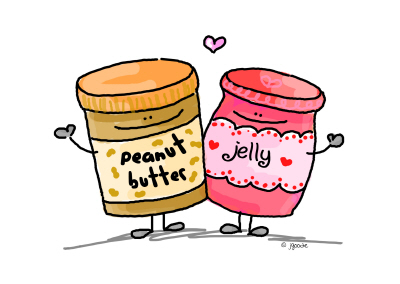
\includegraphics[width=0.6\textwidth]{figures/peanutbutterlover}}
\only<2>{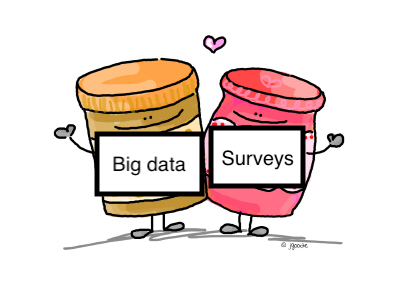
\includegraphics[width=0.6\textwidth]{figures/peanutbutterlover_bigdata_survey}}
\end{center}

\vfill
\tiny{\url{http://schlitterblog.com/wp-content/uploads/2014/05/peanutbutterlover.jpg}}

\end{frame}
%%%%%%%%%%%%%%%%%%%%%%%%%%%
\begin{frame}

\begin{center}
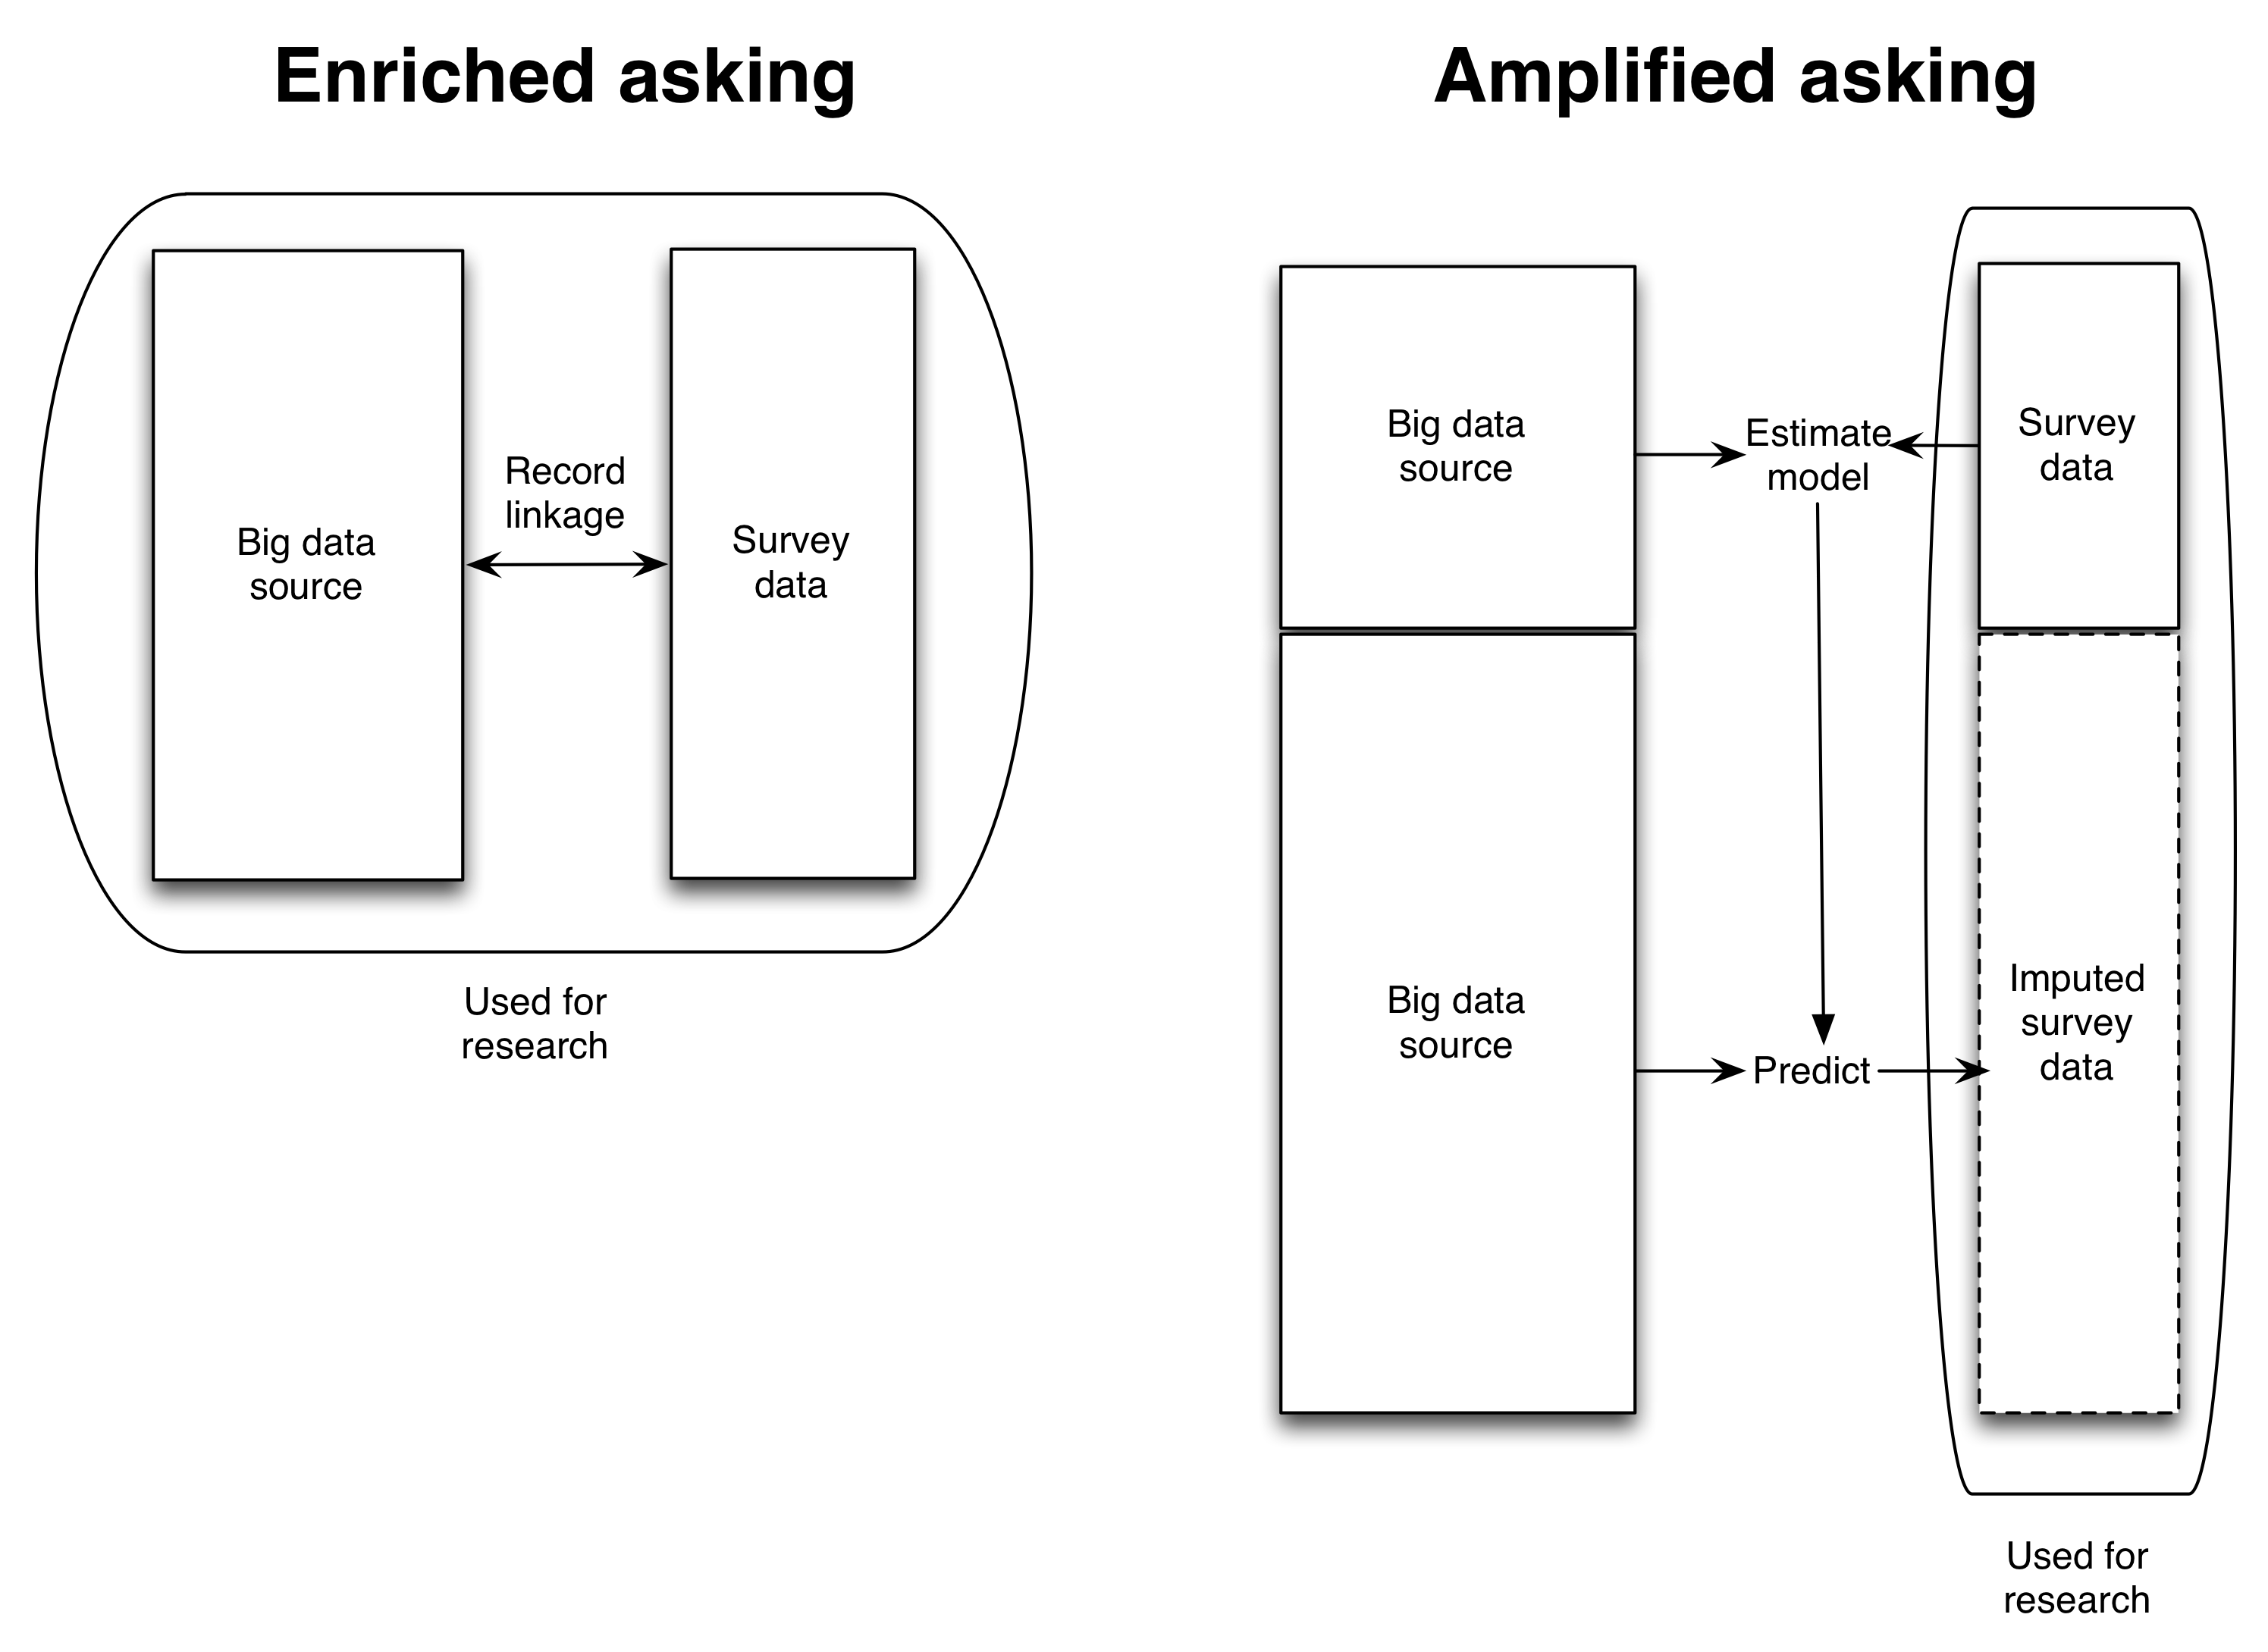
\includegraphics[width=0.6\textwidth]{figures/bitbybit3-12_found_survey_combined}
\end{center}

Note the different role of the big data in each case

\end{frame}
%%%%%%%%%%%%%%%%%%%%%%%%%%%
\begin{frame}

\begin{center}
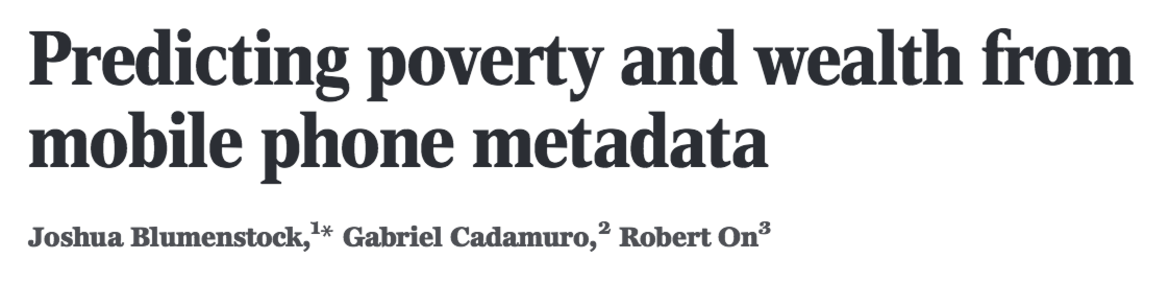
\includegraphics[width=0.9\textwidth]{figures/blumenstock_predicting_2015_title}
\end{center}

\vfill
\url{http://dx.doi.org/10.1126/science.aac4420}
\end{frame}
%%%%%%%%%%%%%%%%%%%%%%%%%%%
\begin{frame}

\begin{center}
\only<1>{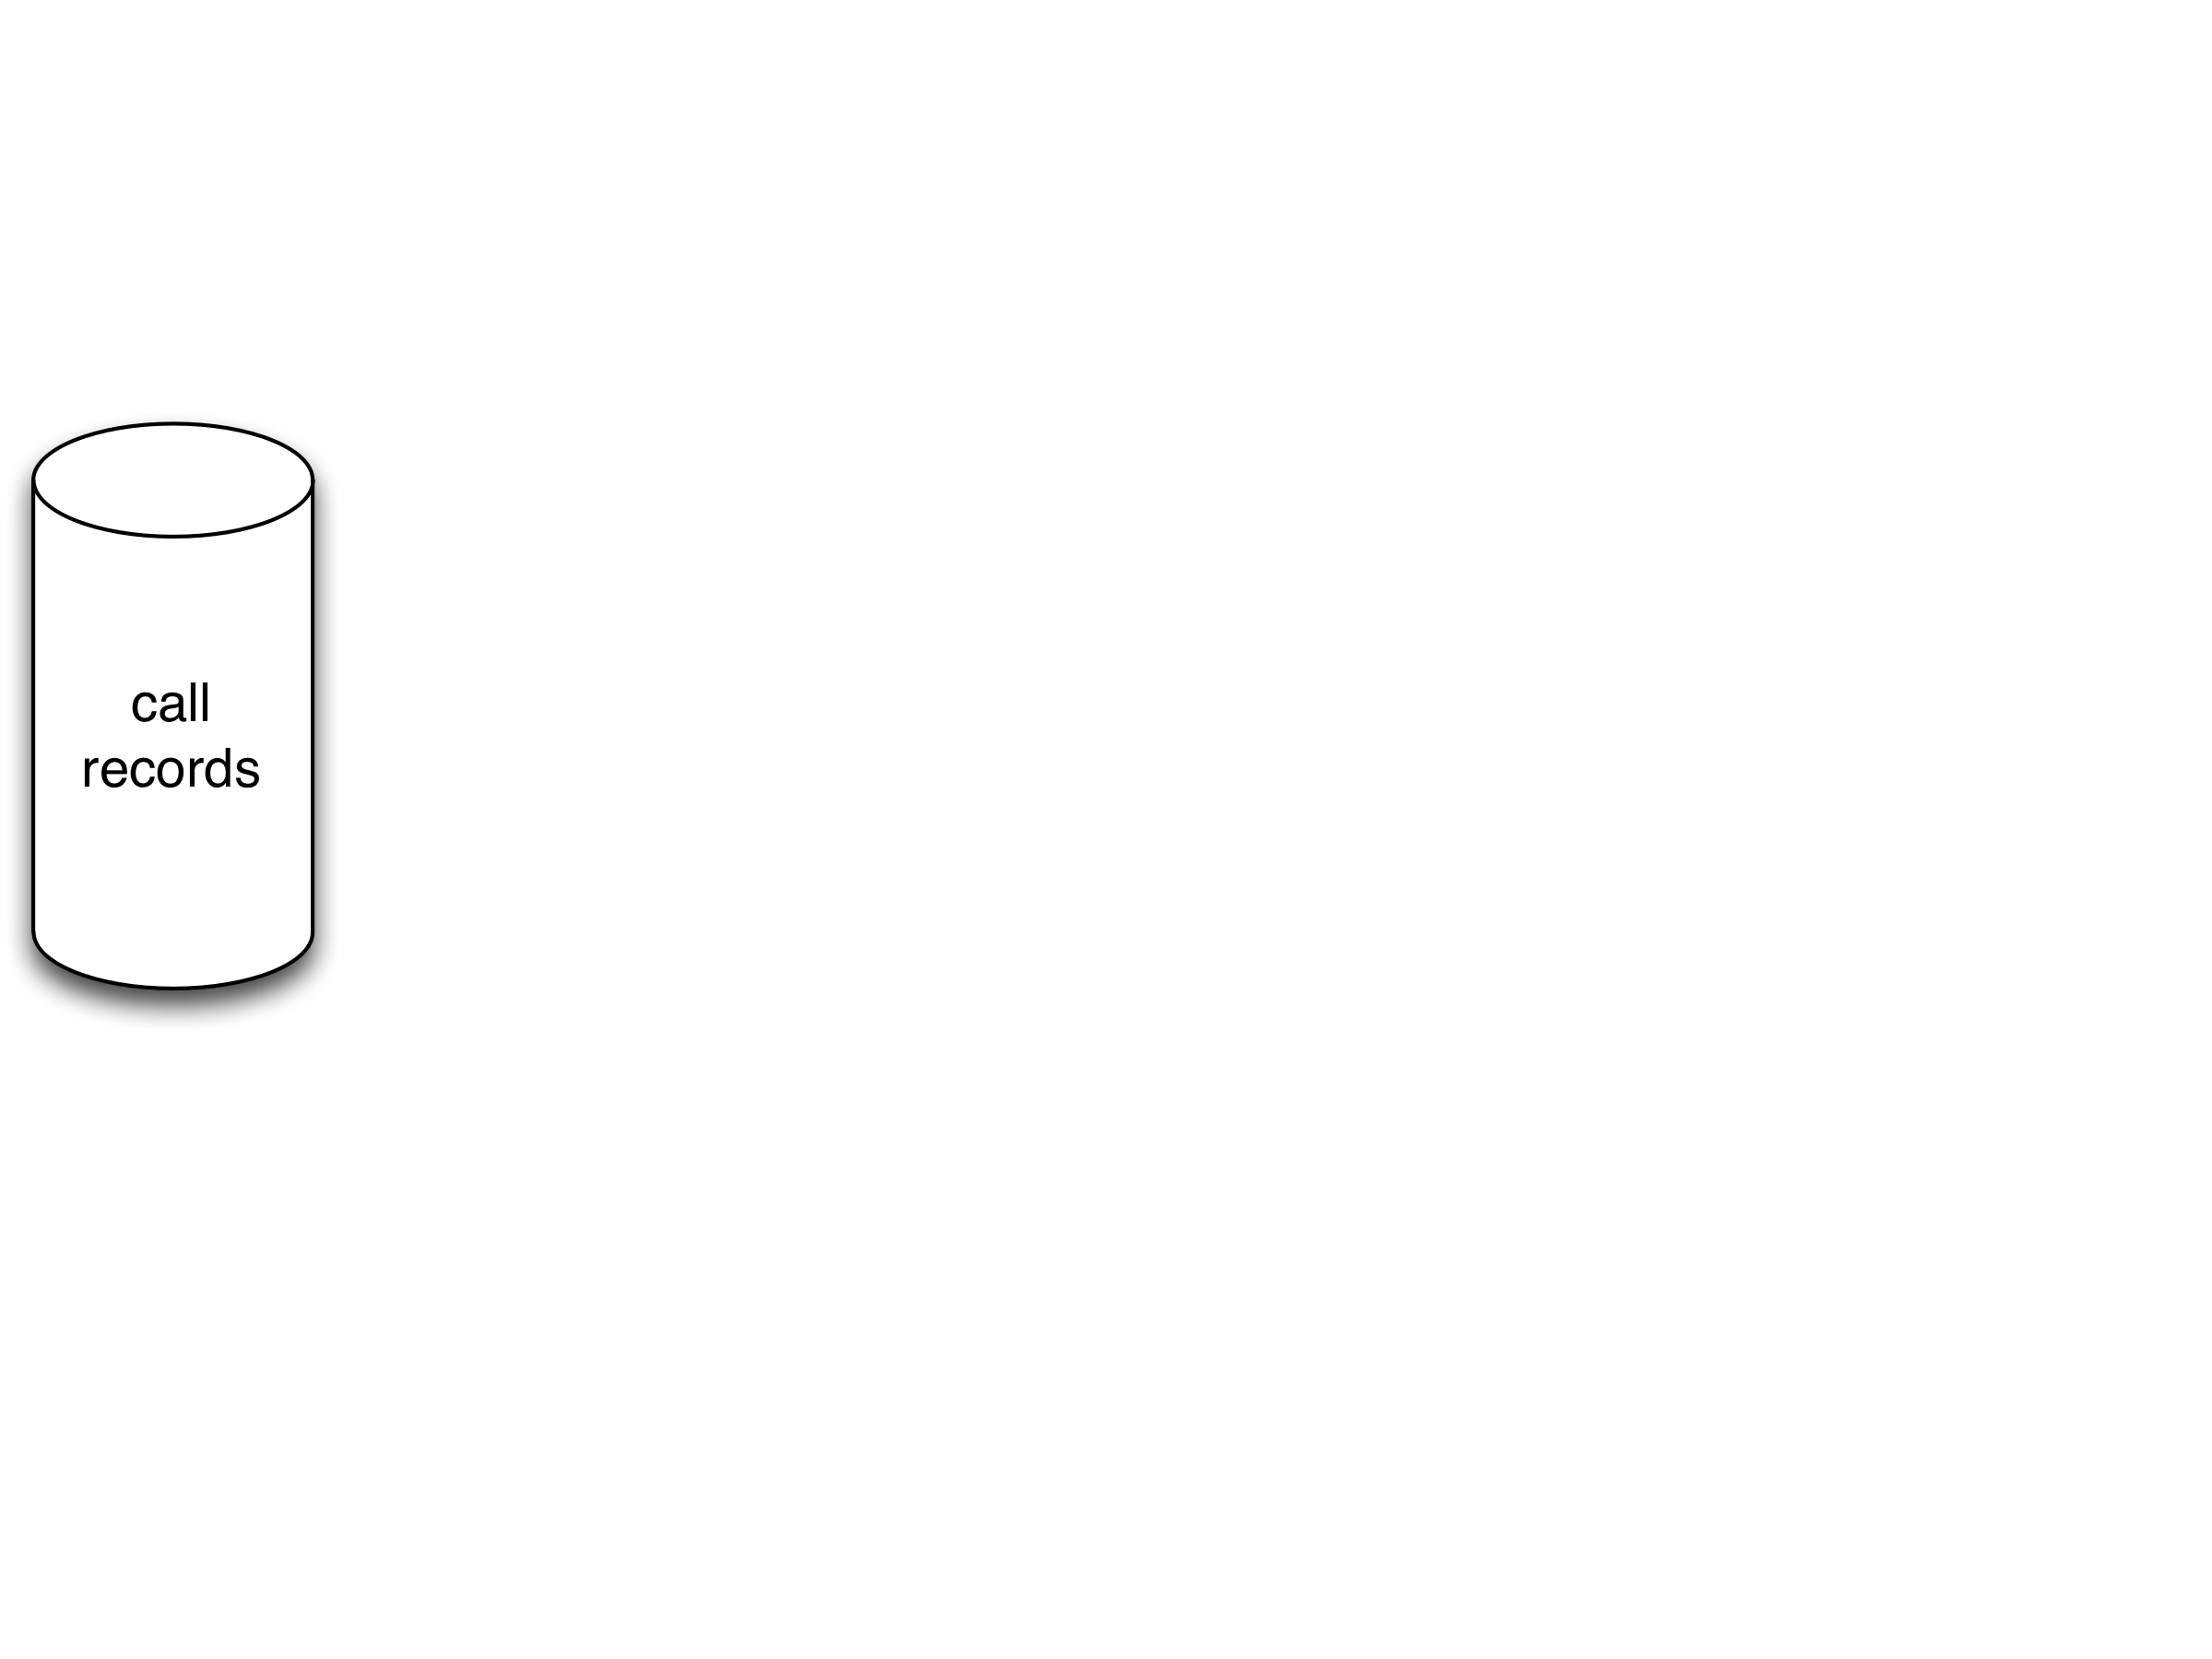
\includegraphics[width=0.7\textwidth]{figures/blumenstock_predicting_2015_schematic_1}}
\only<2>{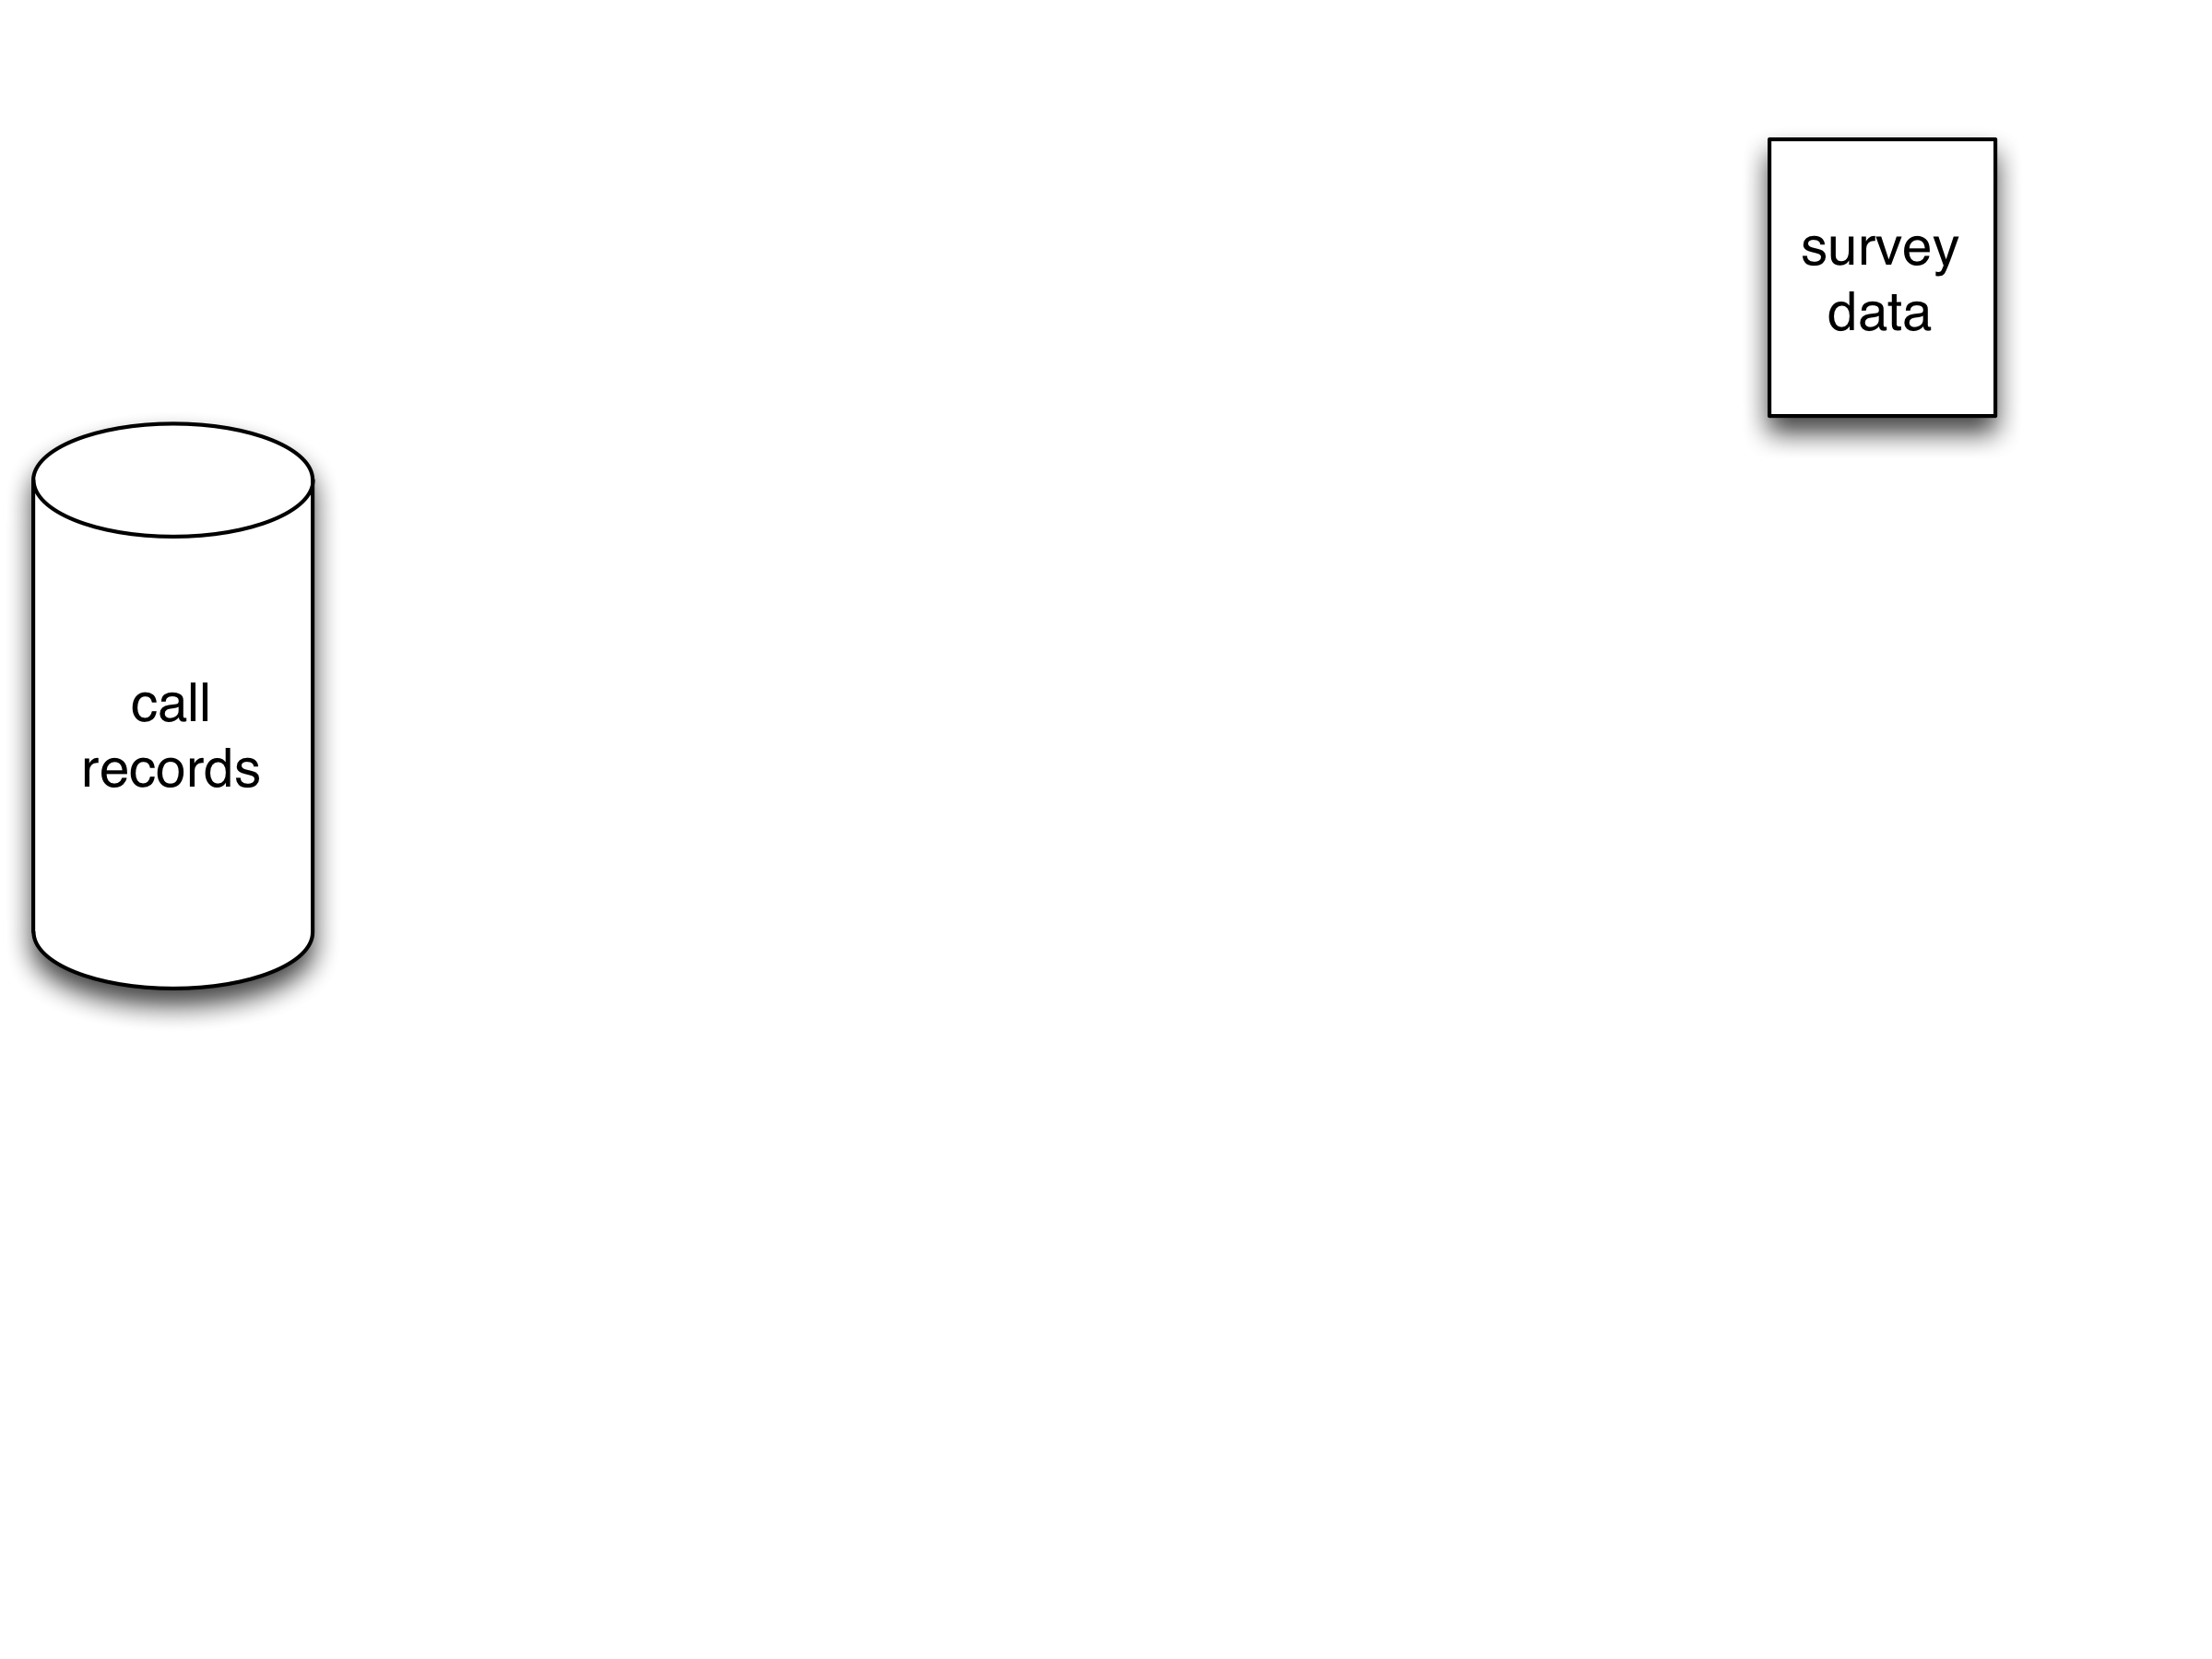
\includegraphics[width=0.7\textwidth]{figures/blumenstock_predicting_2015_schematic_2}}
\only<3>{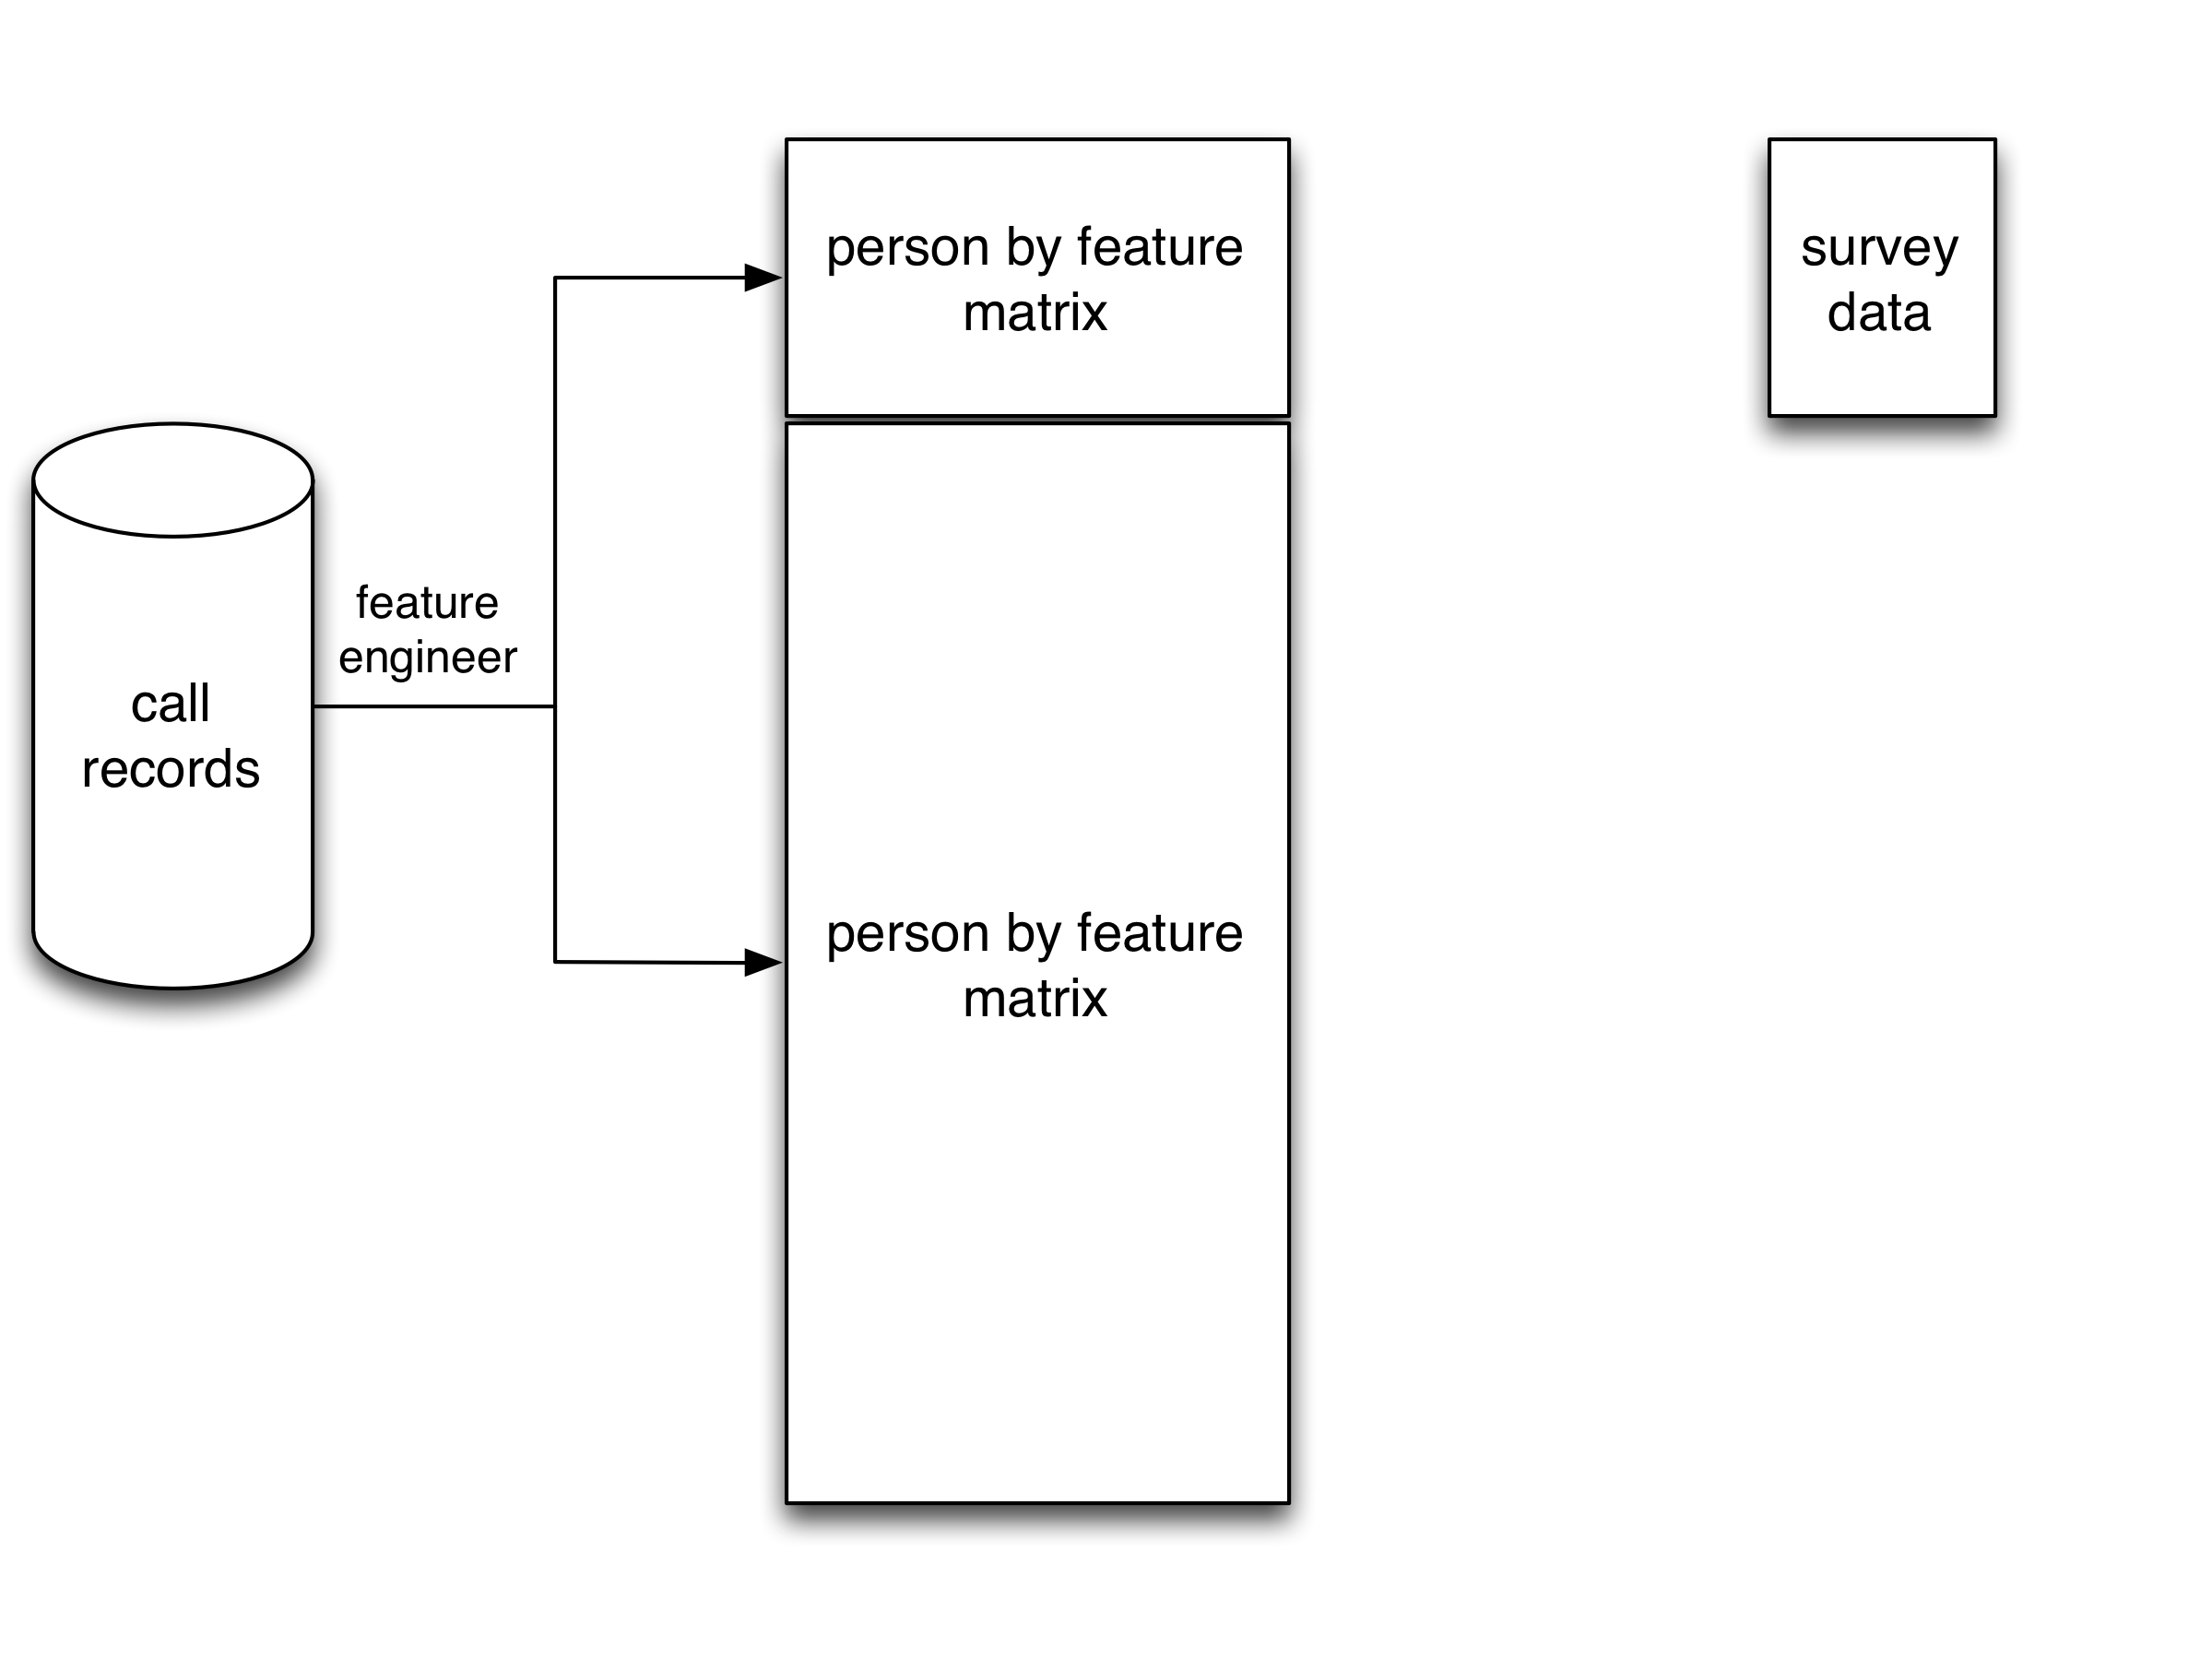
\includegraphics[width=0.7\textwidth]{figures/blumenstock_predicting_2015_schematic_3}}
\only<4>{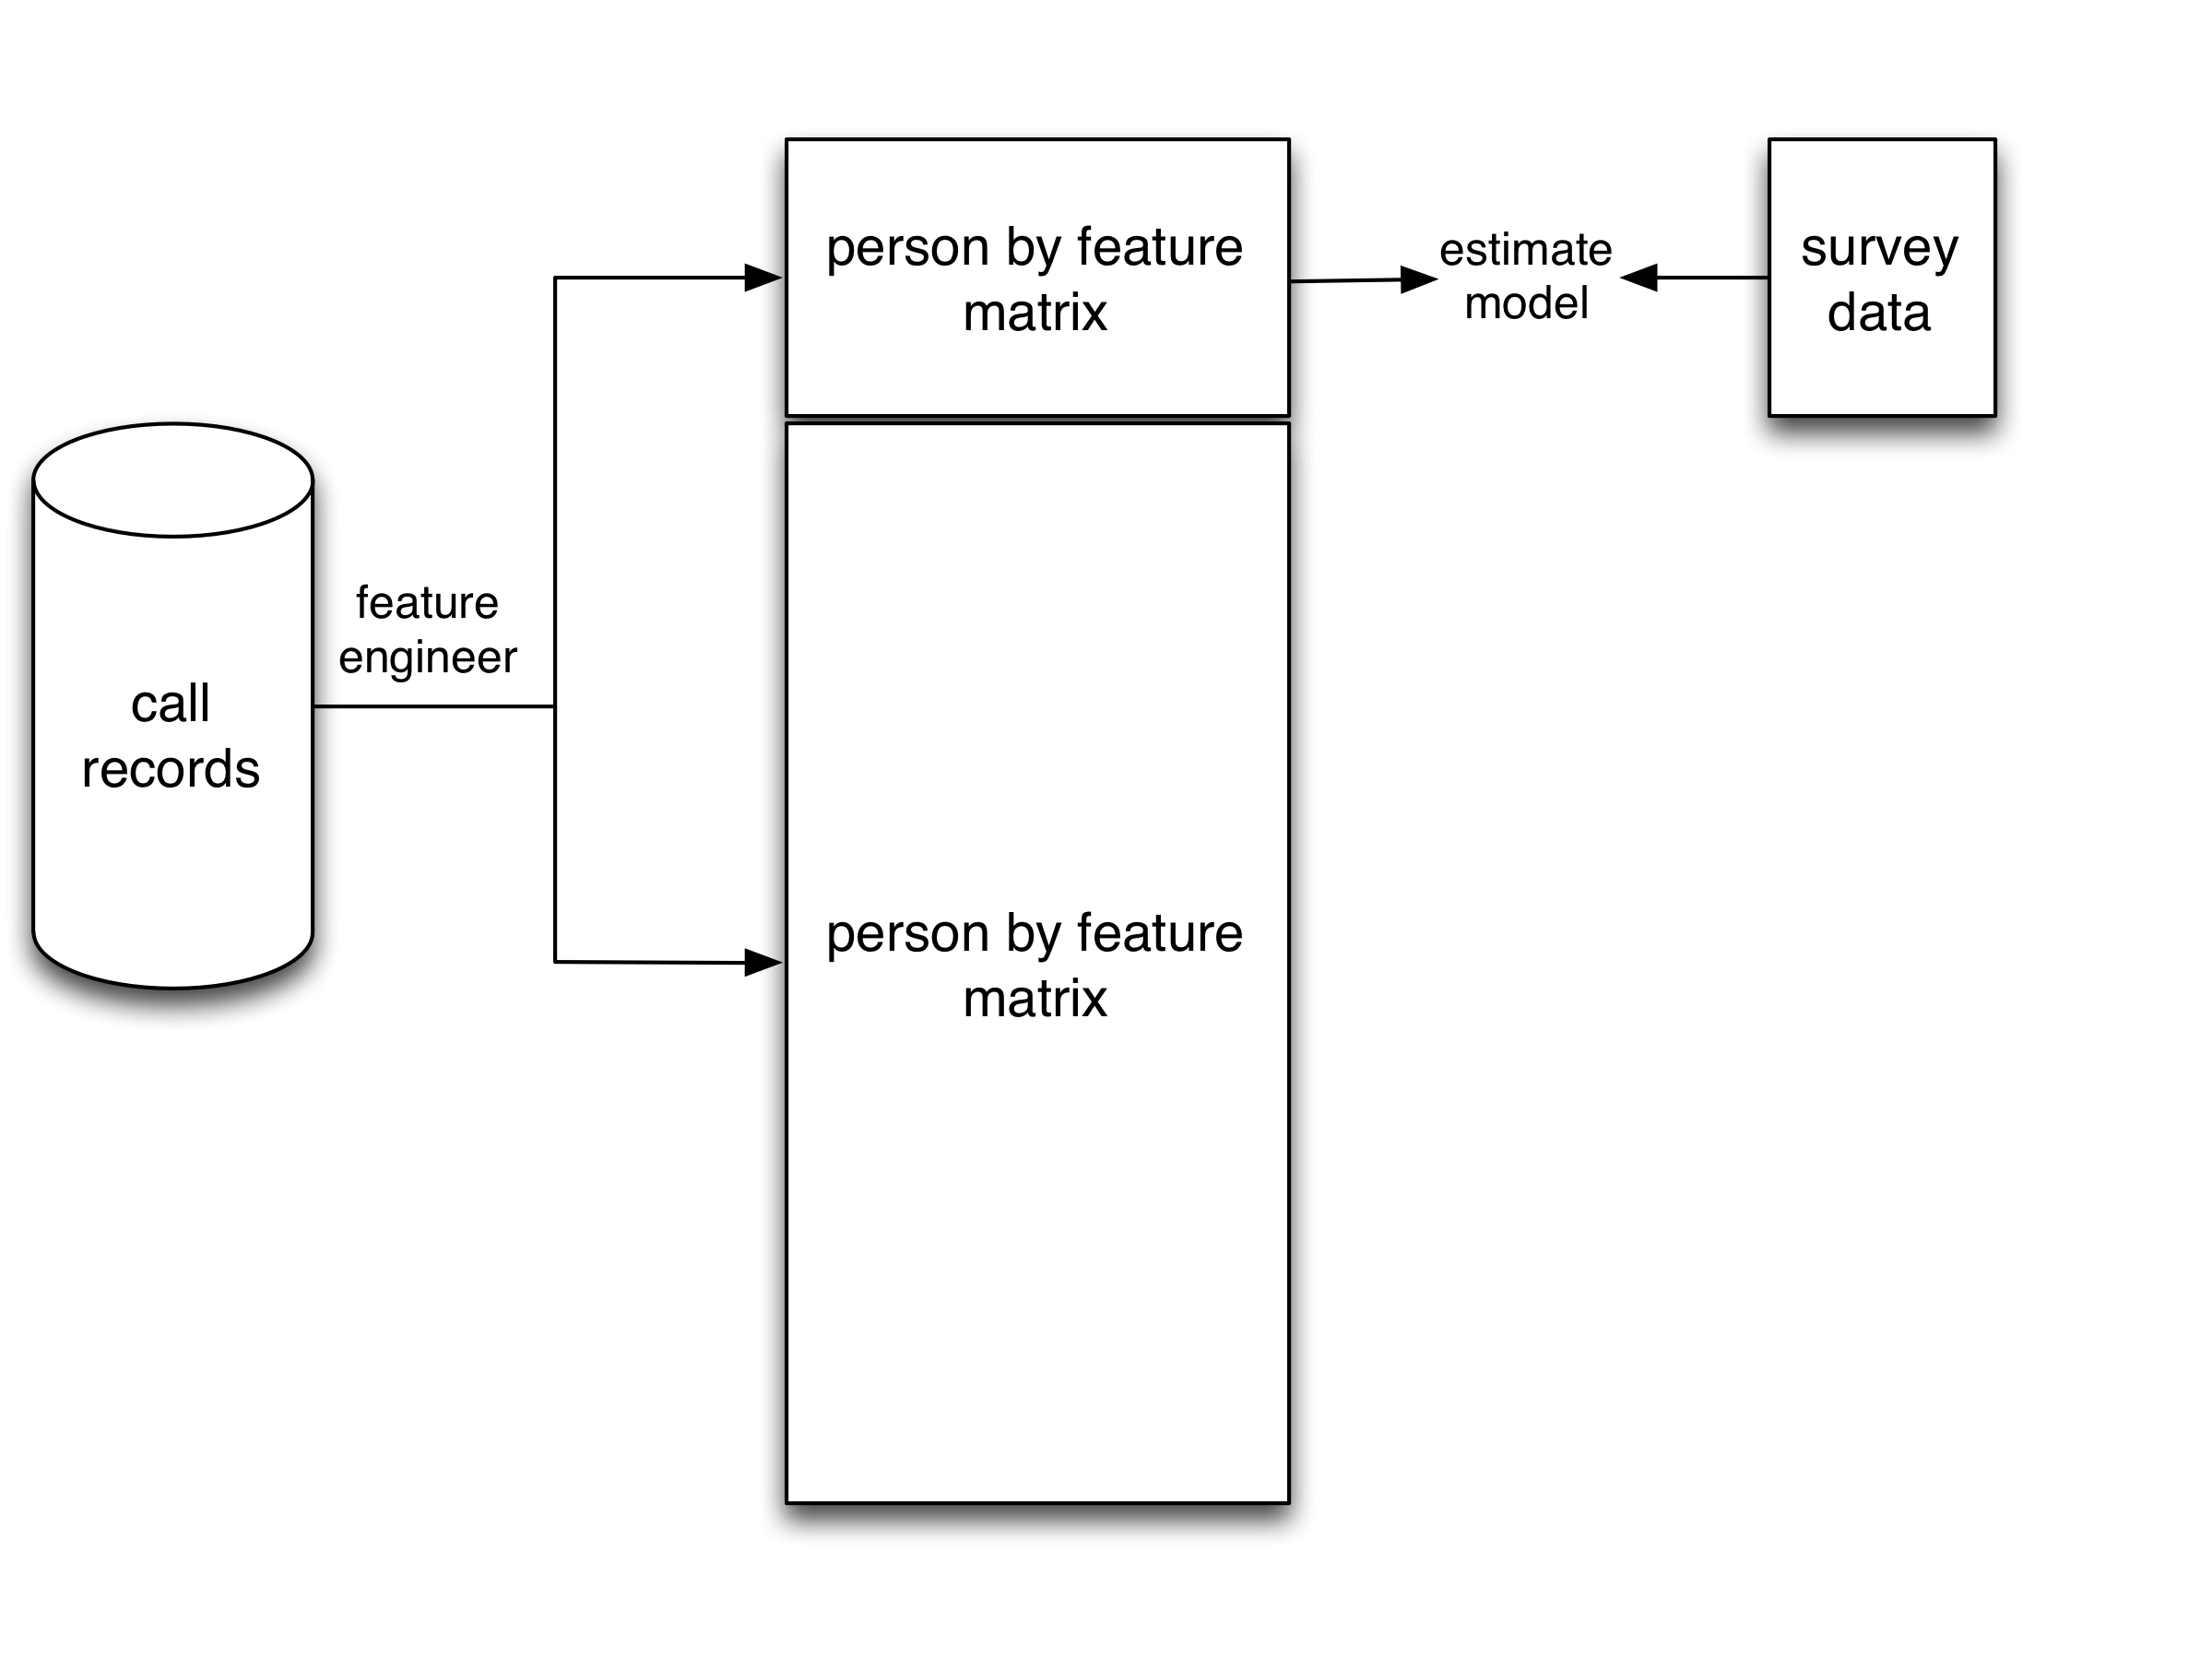
\includegraphics[width=0.7\textwidth]{figures/blumenstock_predicting_2015_schematic_4}}
\only<5>{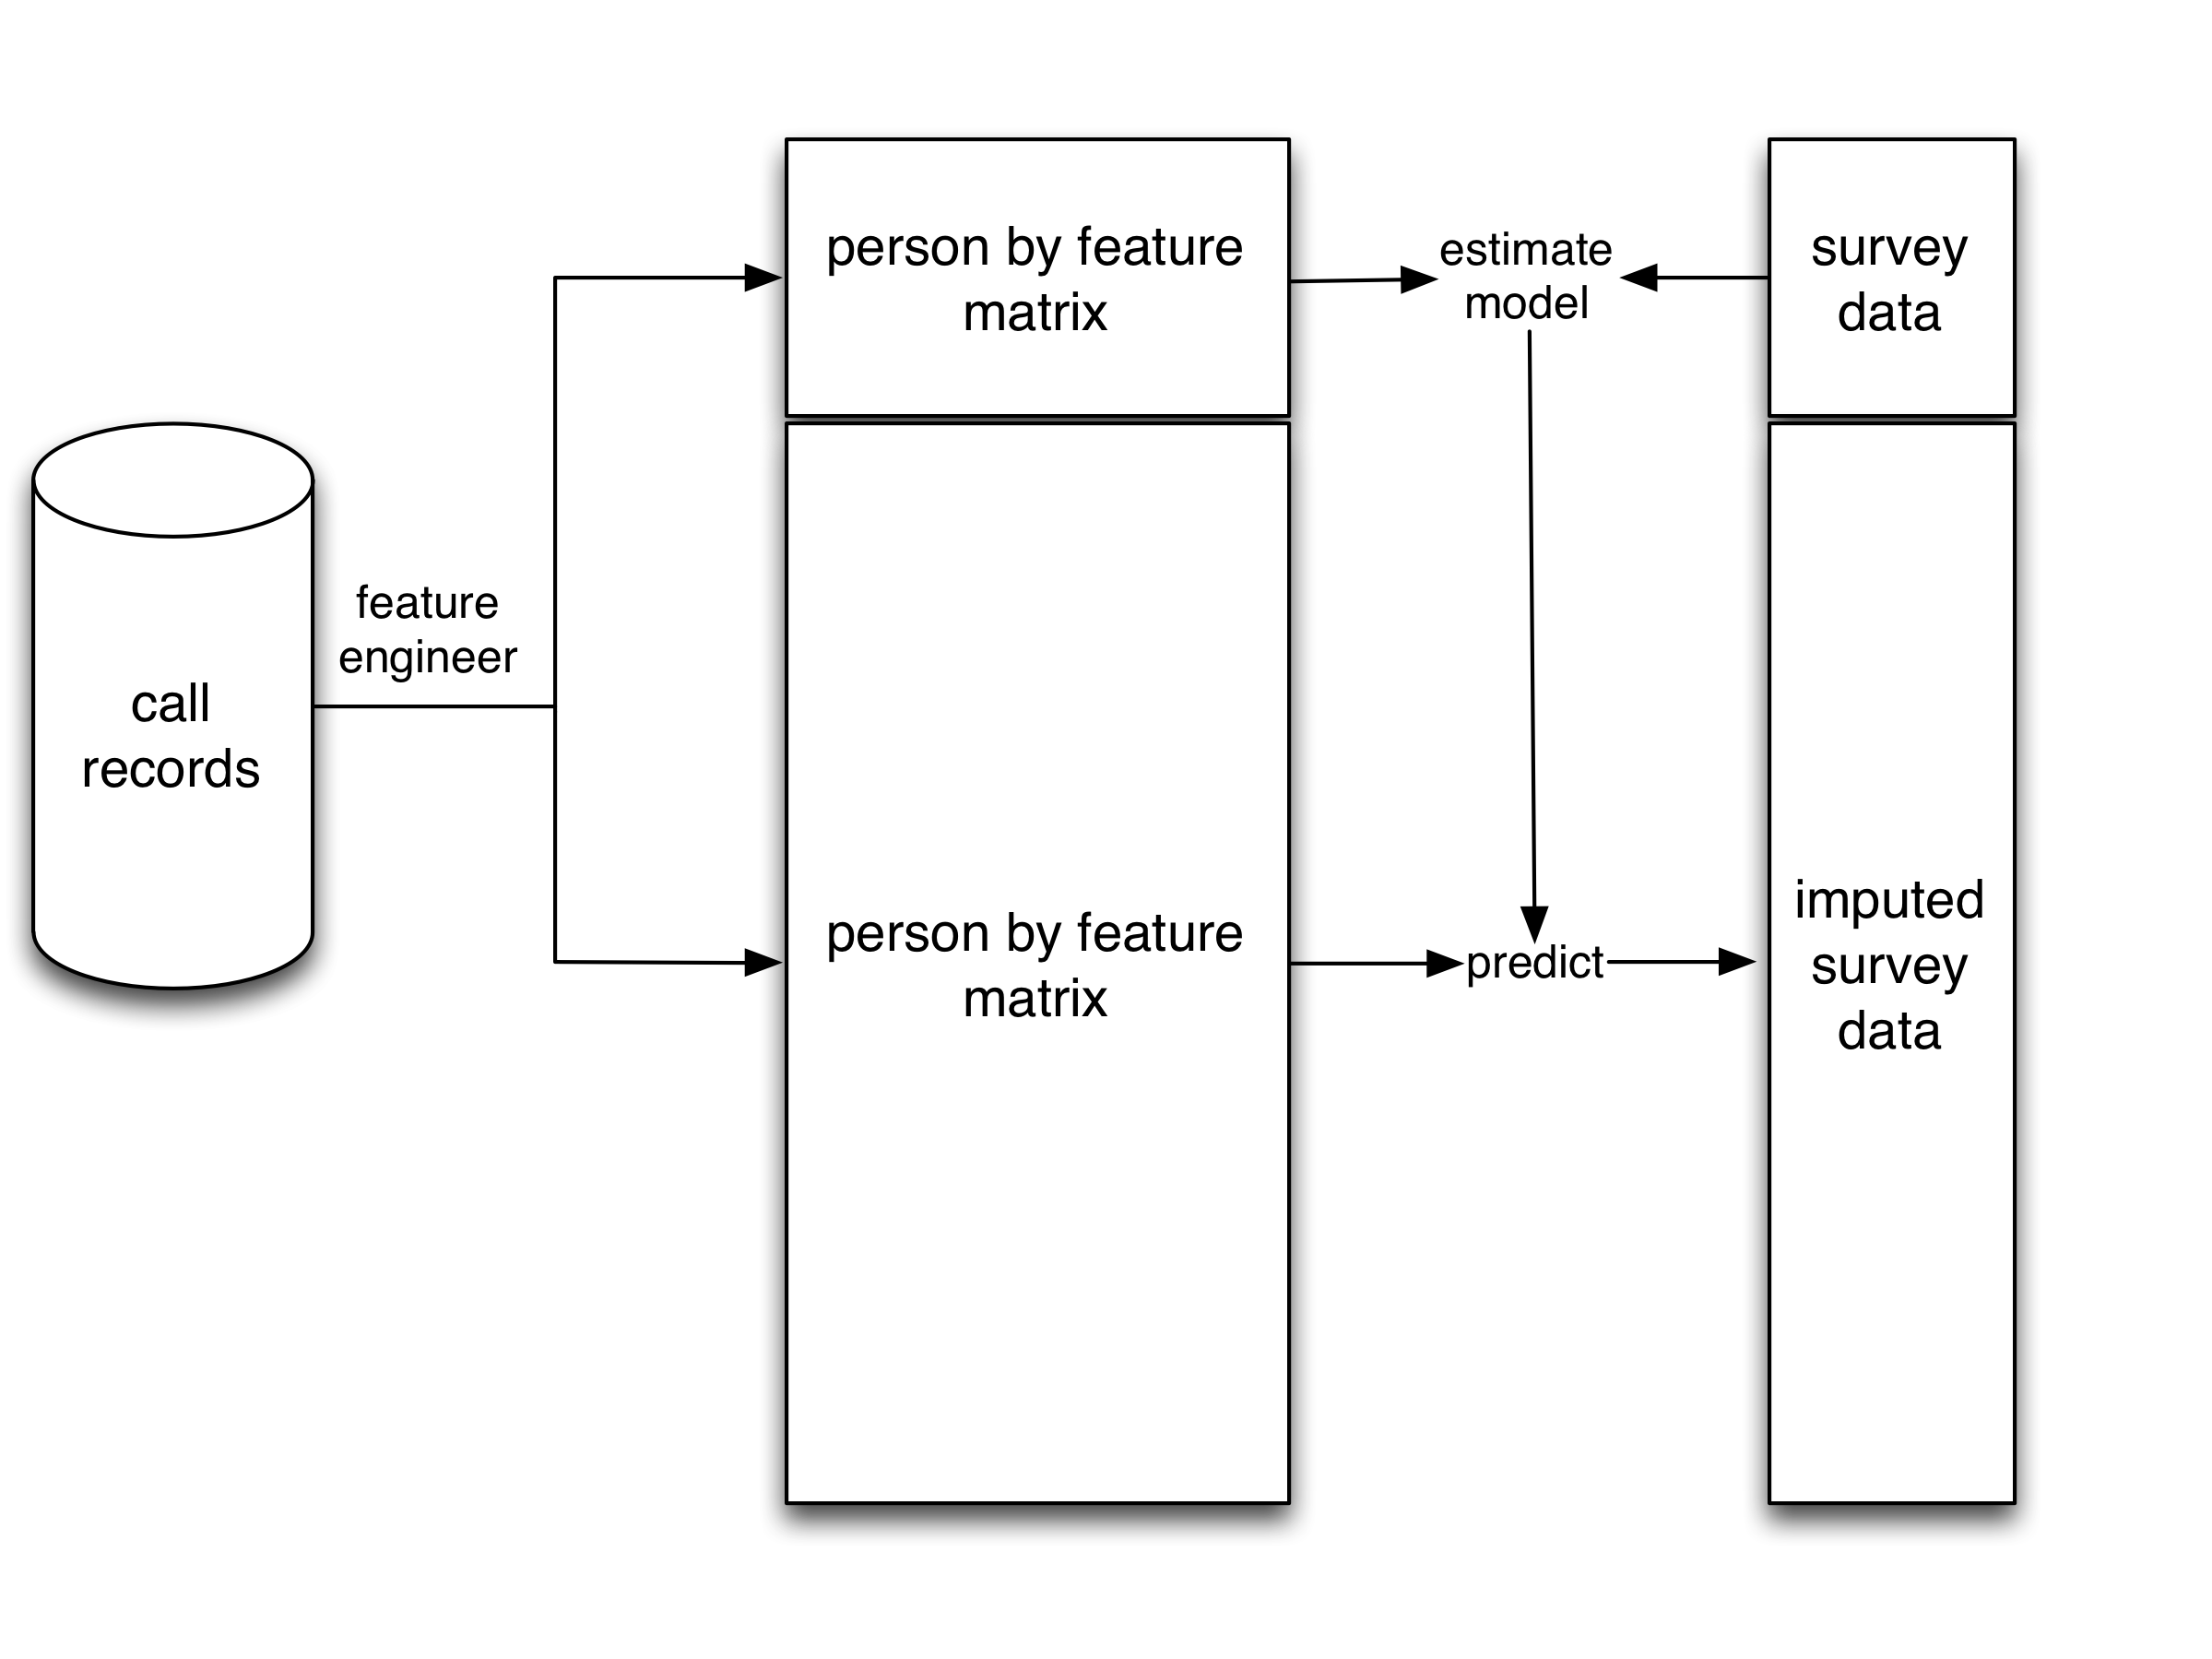
\includegraphics[width=0.7\textwidth]{figures/blumenstock_predicting_2015_schematic_5}}
\only<6>{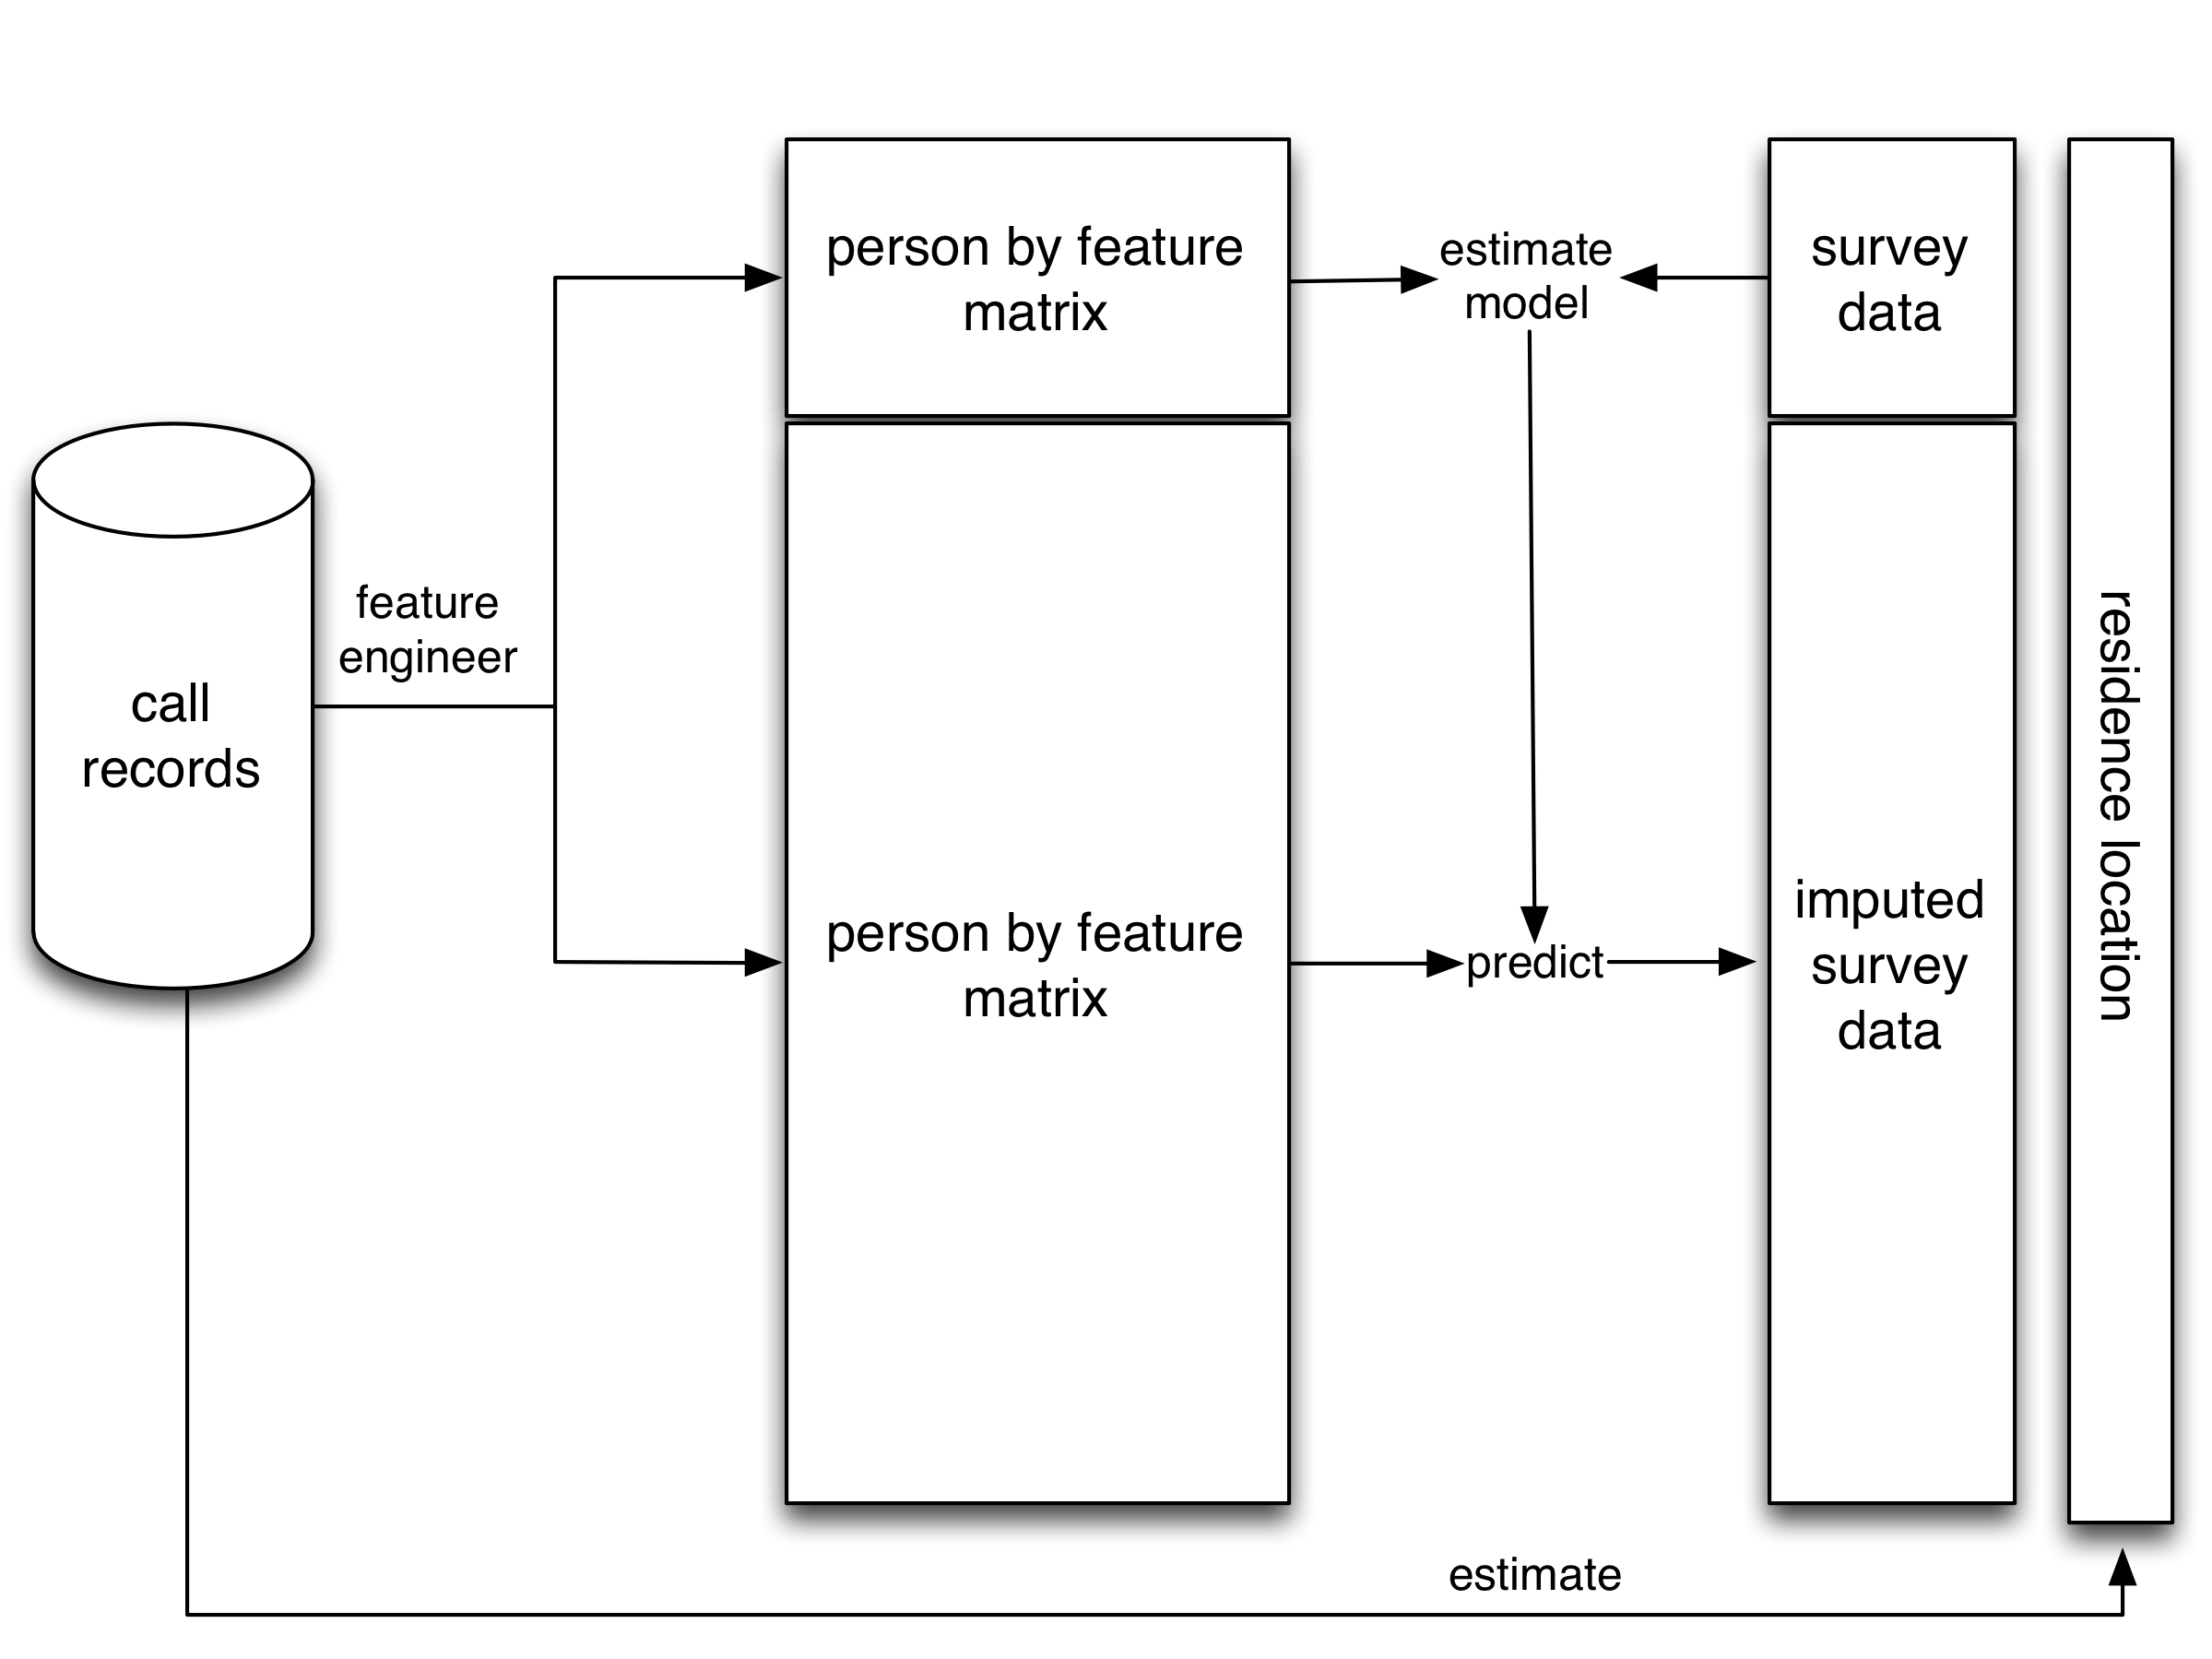
\includegraphics[width=0.7\textwidth]{figures/blumenstock_predicting_2015_schematic_6}}
\end{center}

\end{frame}
%%%%%%%%%%%%%%%%%%%%%%%%%%%
\begin{frame}

\begin{center}
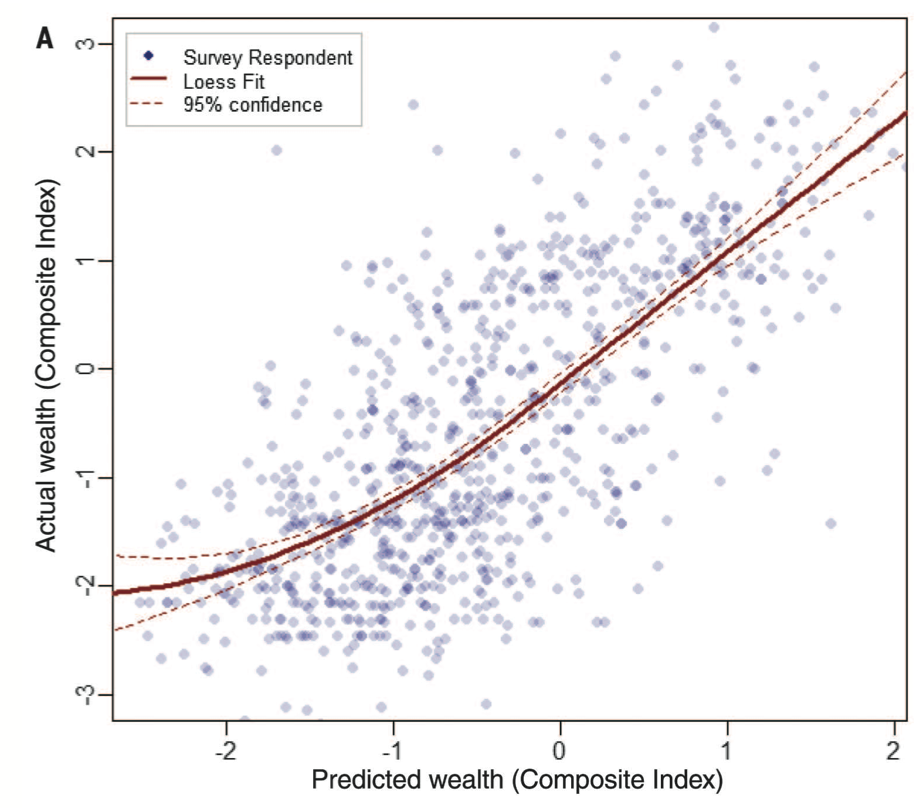
\includegraphics[width=0.7\textwidth]{figures/blumenstock_predicting_2015_fig1a}
\end{center}

\end{frame}
%%%%%%%%%%%%%%%%%%%%%%%%%%
\begin{frame}

\begin{center}
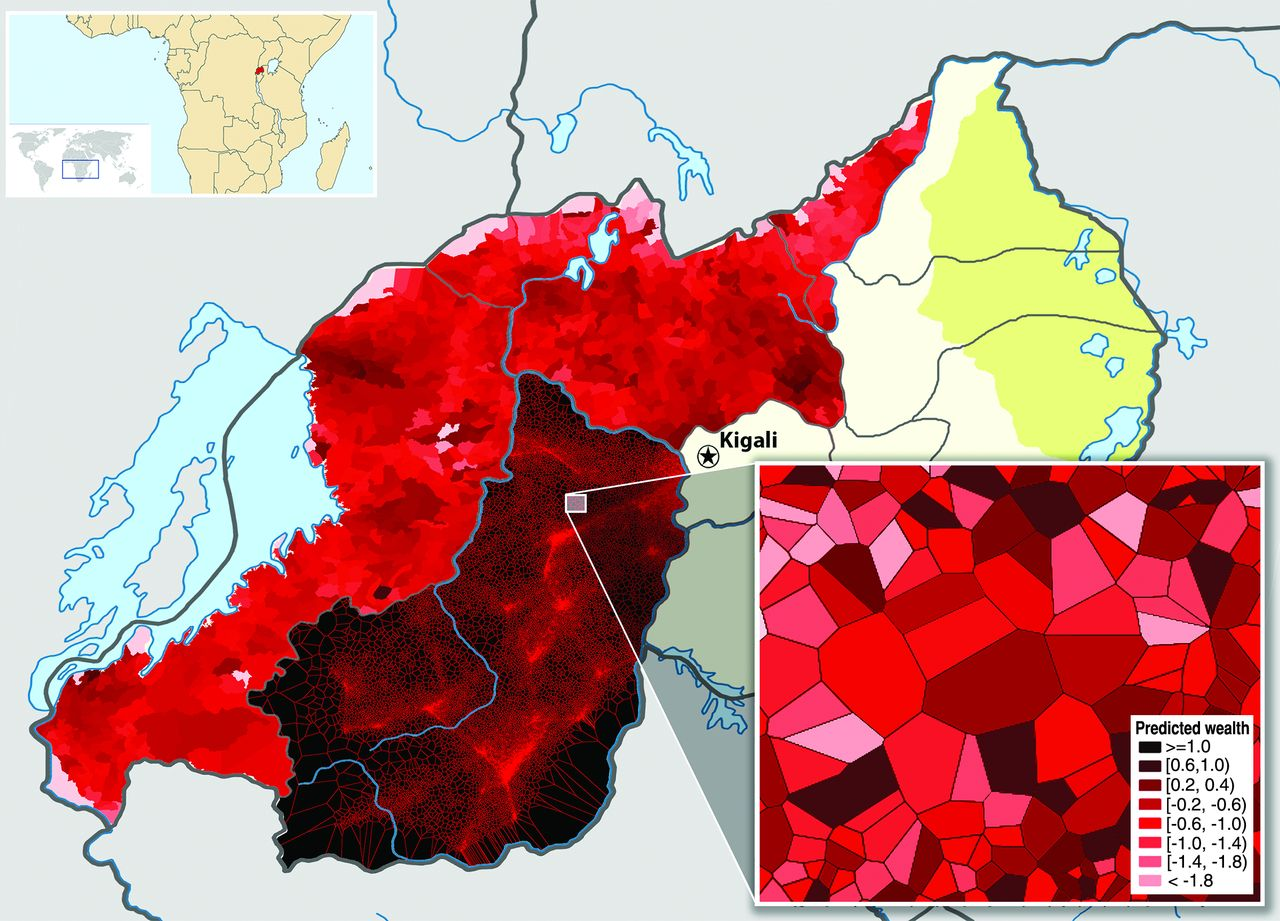
\includegraphics[width=0.7\textwidth]{figures/blumenstock_predicting_2015_fig2}
\end{center}

\end{frame}
%%%%%%%%%%%%%%%%%%%%%%%%%%
\begin{frame}

\begin{center}
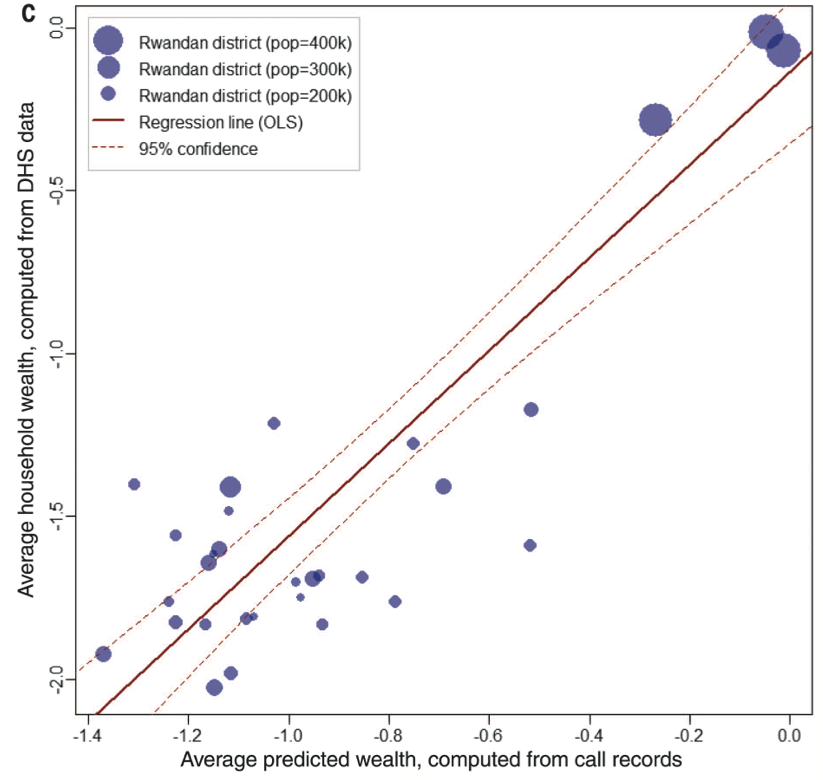
\includegraphics[width=0.45\textwidth]{figures/blumenstock_predicting_2015_fig3c}
\end{center}

\pause

\begin{itemize}
\item 10 times faster
\item 50 times cheaper
\end{itemize}

\end{frame}
%%%%%%%%%%%%%%%%%%%%%%%%%%
\begin{frame}

\begin{center}
\begin{tabular}{ccc}
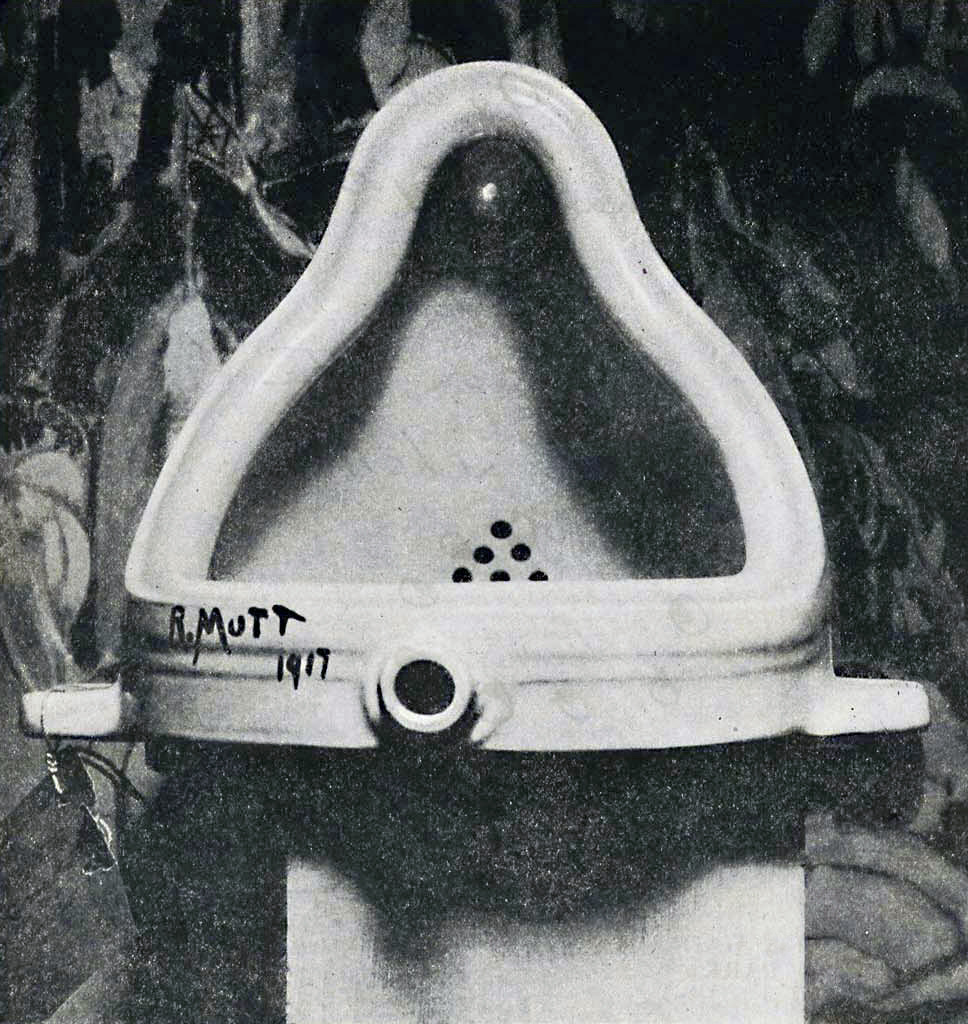
\includegraphics[width=0.30\textwidth]{figures/duchamp_fountain} & \phantom{12} \LARGE{+} \phantom{12} & 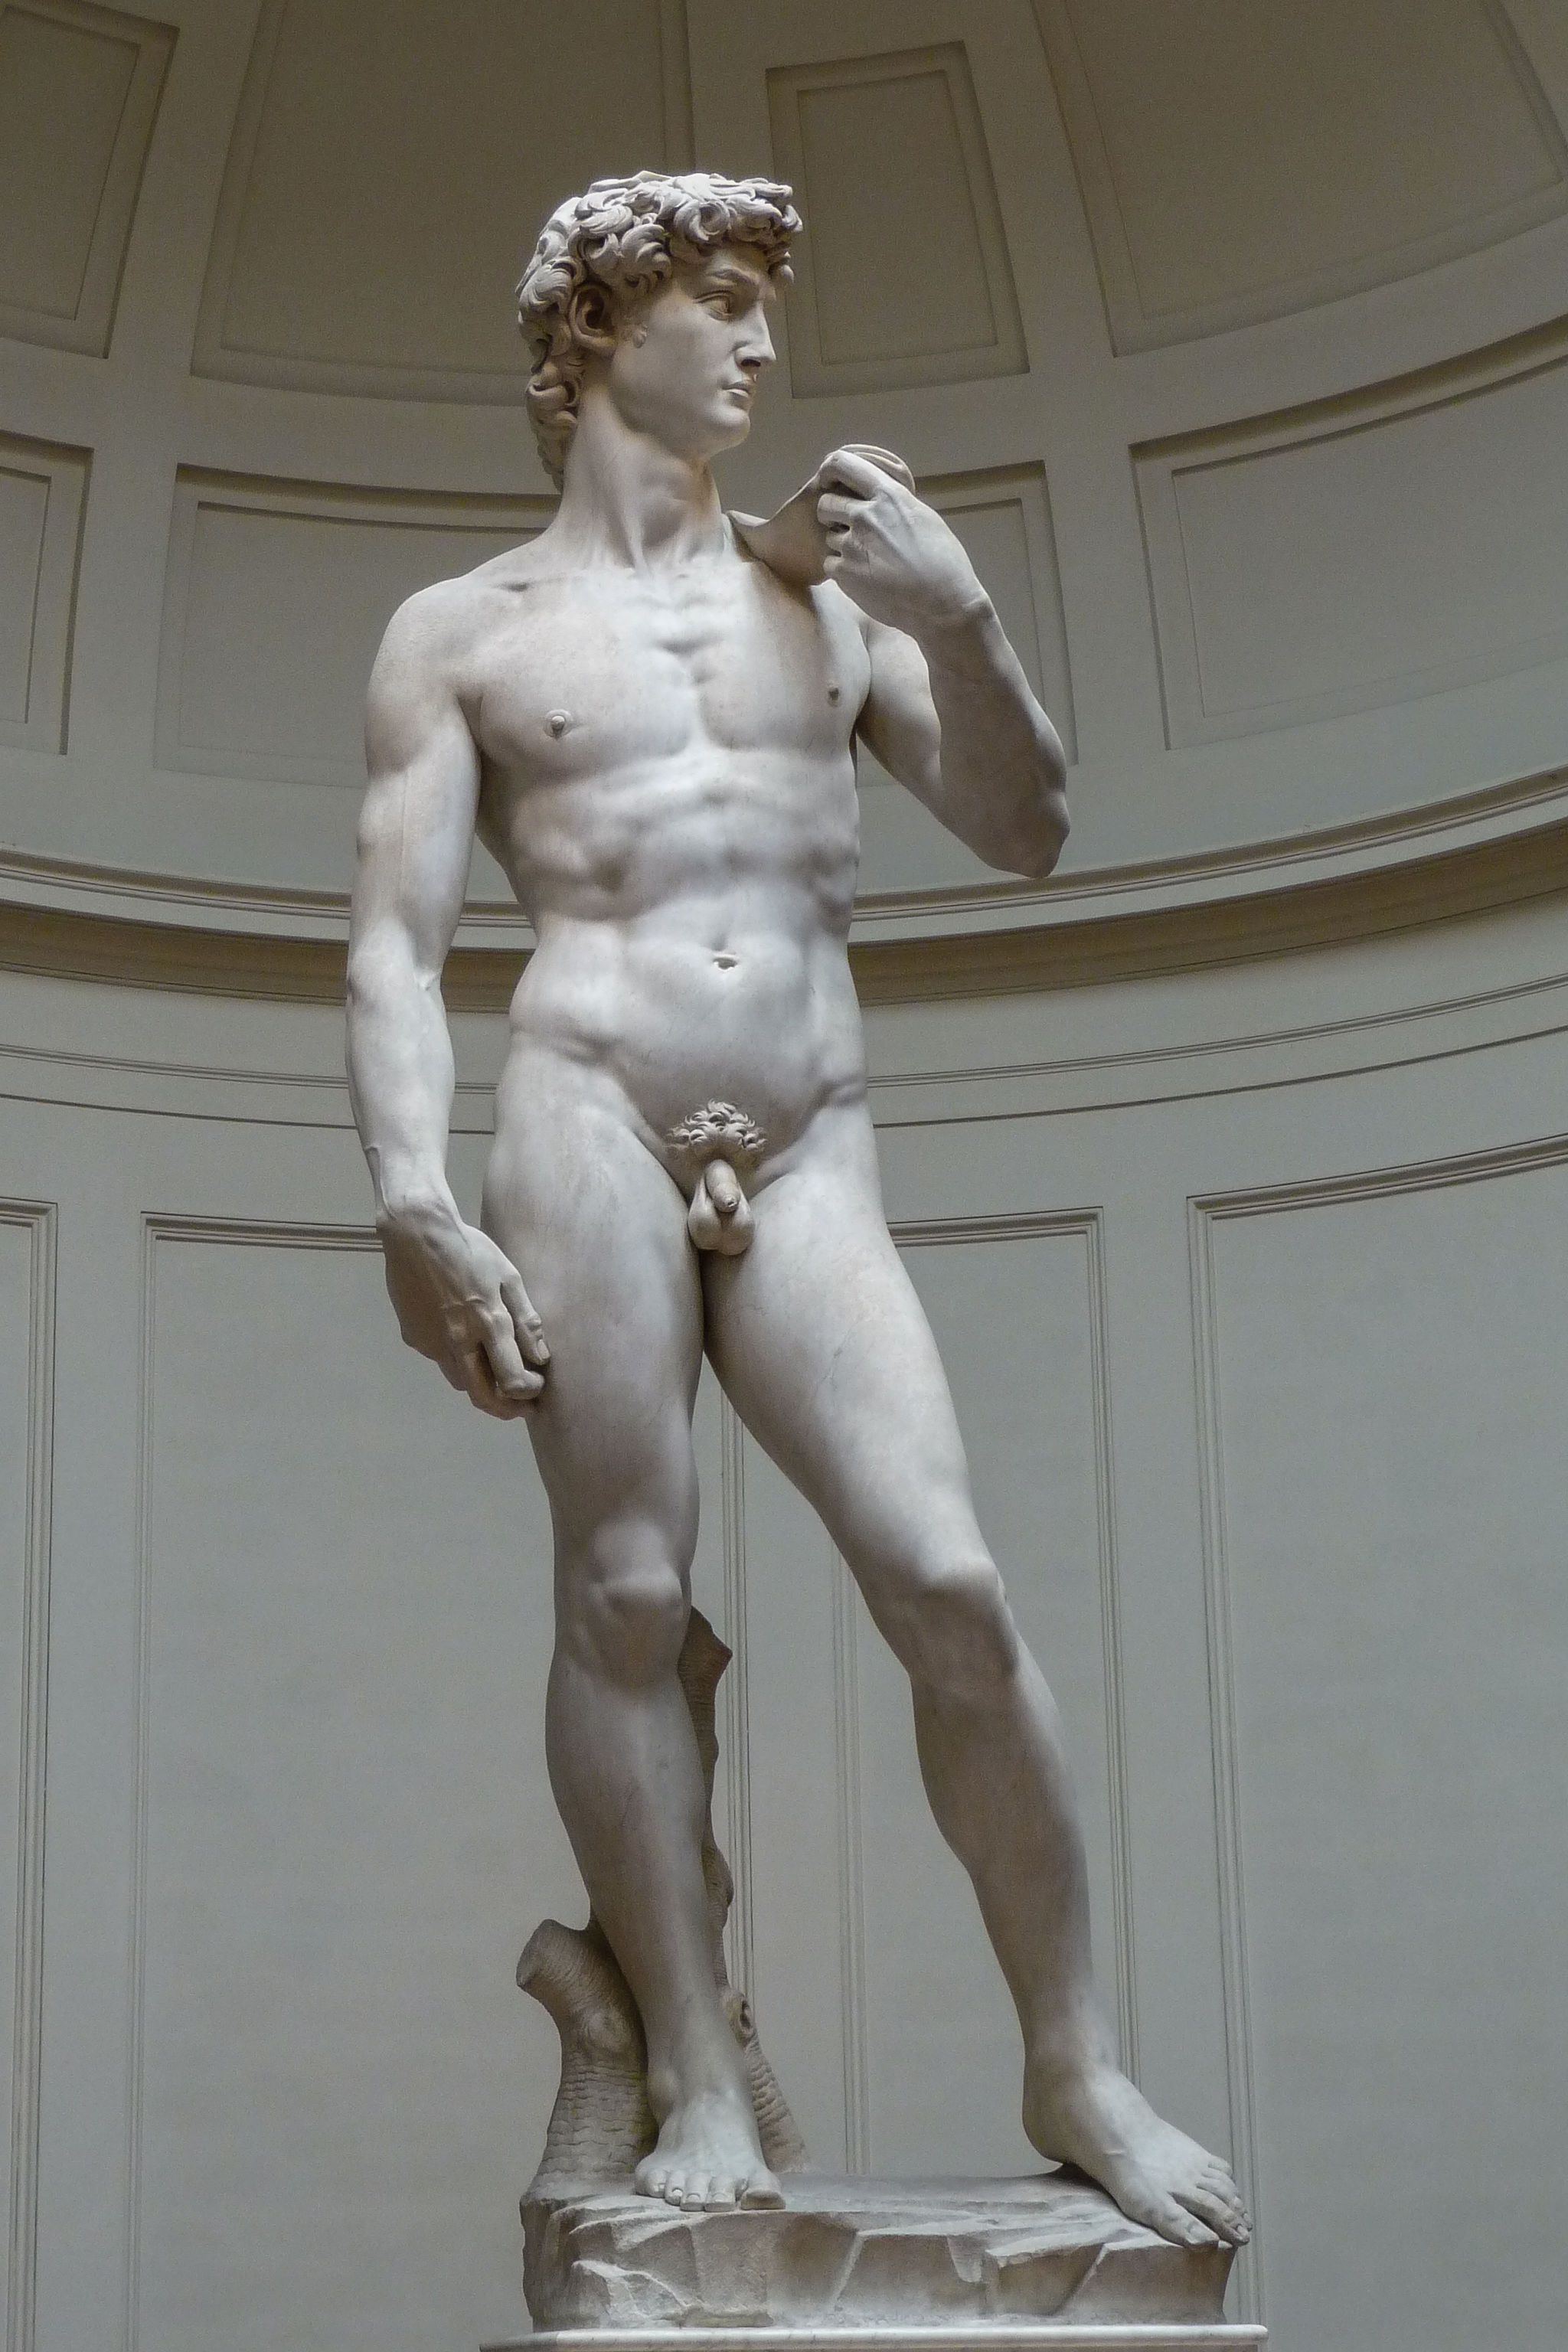
\includegraphics[width=0.30\textwidth]{figures/michelangelo_david} \\
\LARGE{Readymades} &  & \LARGE{Custommades}
\end{tabular}
\end{center}

\vfill
\vspace{0.2in}
\TINY{\url{https://commons.wikimedia.org/wiki/File:Duchamp_Fountaine.jpg}}\\
\TINY{\url{https://commons.wikimedia.org/wiki/File:\%27David\%27_by_Michelangelo_JBU0001.JPG}}

\end{frame}
%%%%%%%%%%%%%%%%%%%%%%%%%%%
{
\usebackgroundtemplate{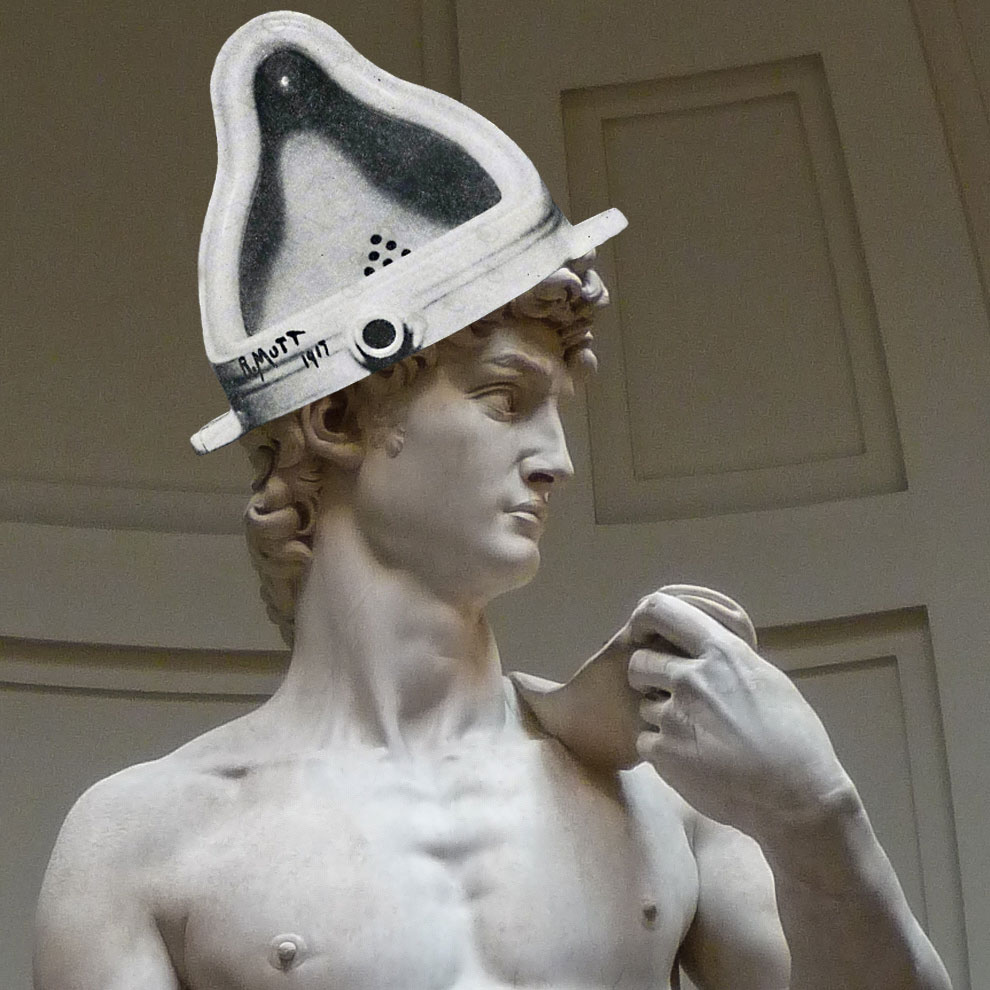
\includegraphics[width=\paperwidth]{figures/custom-david-cropped}}
\begin{frame}[plain]

\vspace{3.58in}
\hspace{-0.32in}
\TINY{Created by Kedron Rhodes}
\end{frame}
}
%%%%%%%%%%%%%%%%%%%%%%%%%%
\begin{frame}

\begin{center}
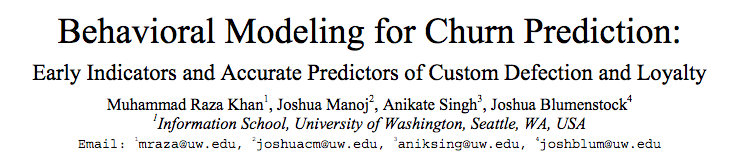
\includegraphics[width=0.3\textwidth]{figures/khan_behavioral_2015_title}
\pause
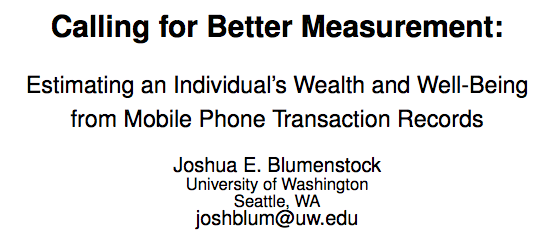
\includegraphics[width=0.3\textwidth]{figures/blumenstock_calling_2014_title}
\pause
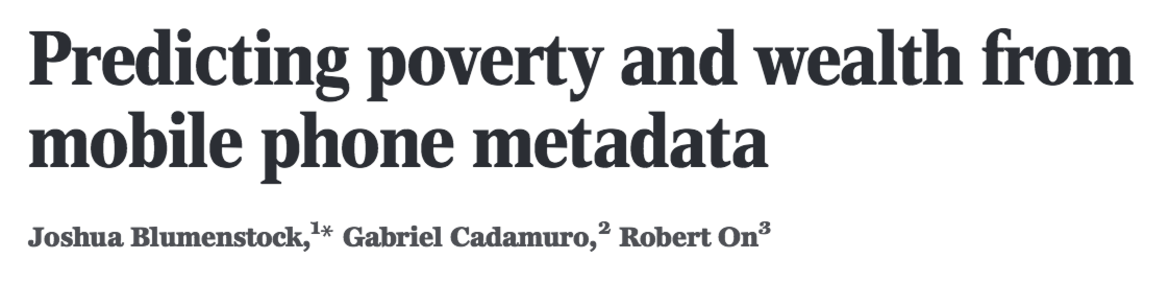
\includegraphics[width=0.3\textwidth]{figures/blumenstock_predicting_2015_title}
\end{center}
\pause
\vfill
The beginning is not the end . . . .
\end{frame}
%%%%%%%%%%%%%%%%%%%%%%%%%%
\begin{frame}

\begin{center}
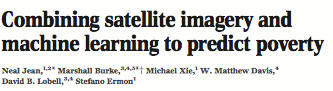
\includegraphics[width=0.8\textwidth]{figures/jean_combining_2016_title}
\end{center}

\vfill

This paper is amazing and surprising (to me).  First a digression . . . .

\end{frame}
%%%%%%%%%%%%%%%%%%%%%%%%
\begin{frame}

Supervised learning:\\
Lots of input-output pairs; goal is to develop a function that will predict the output from the input

\end{frame}
%%%%%%%%%%%%%%%%%%%%%%%%
\begin{frame}

\begin{center}
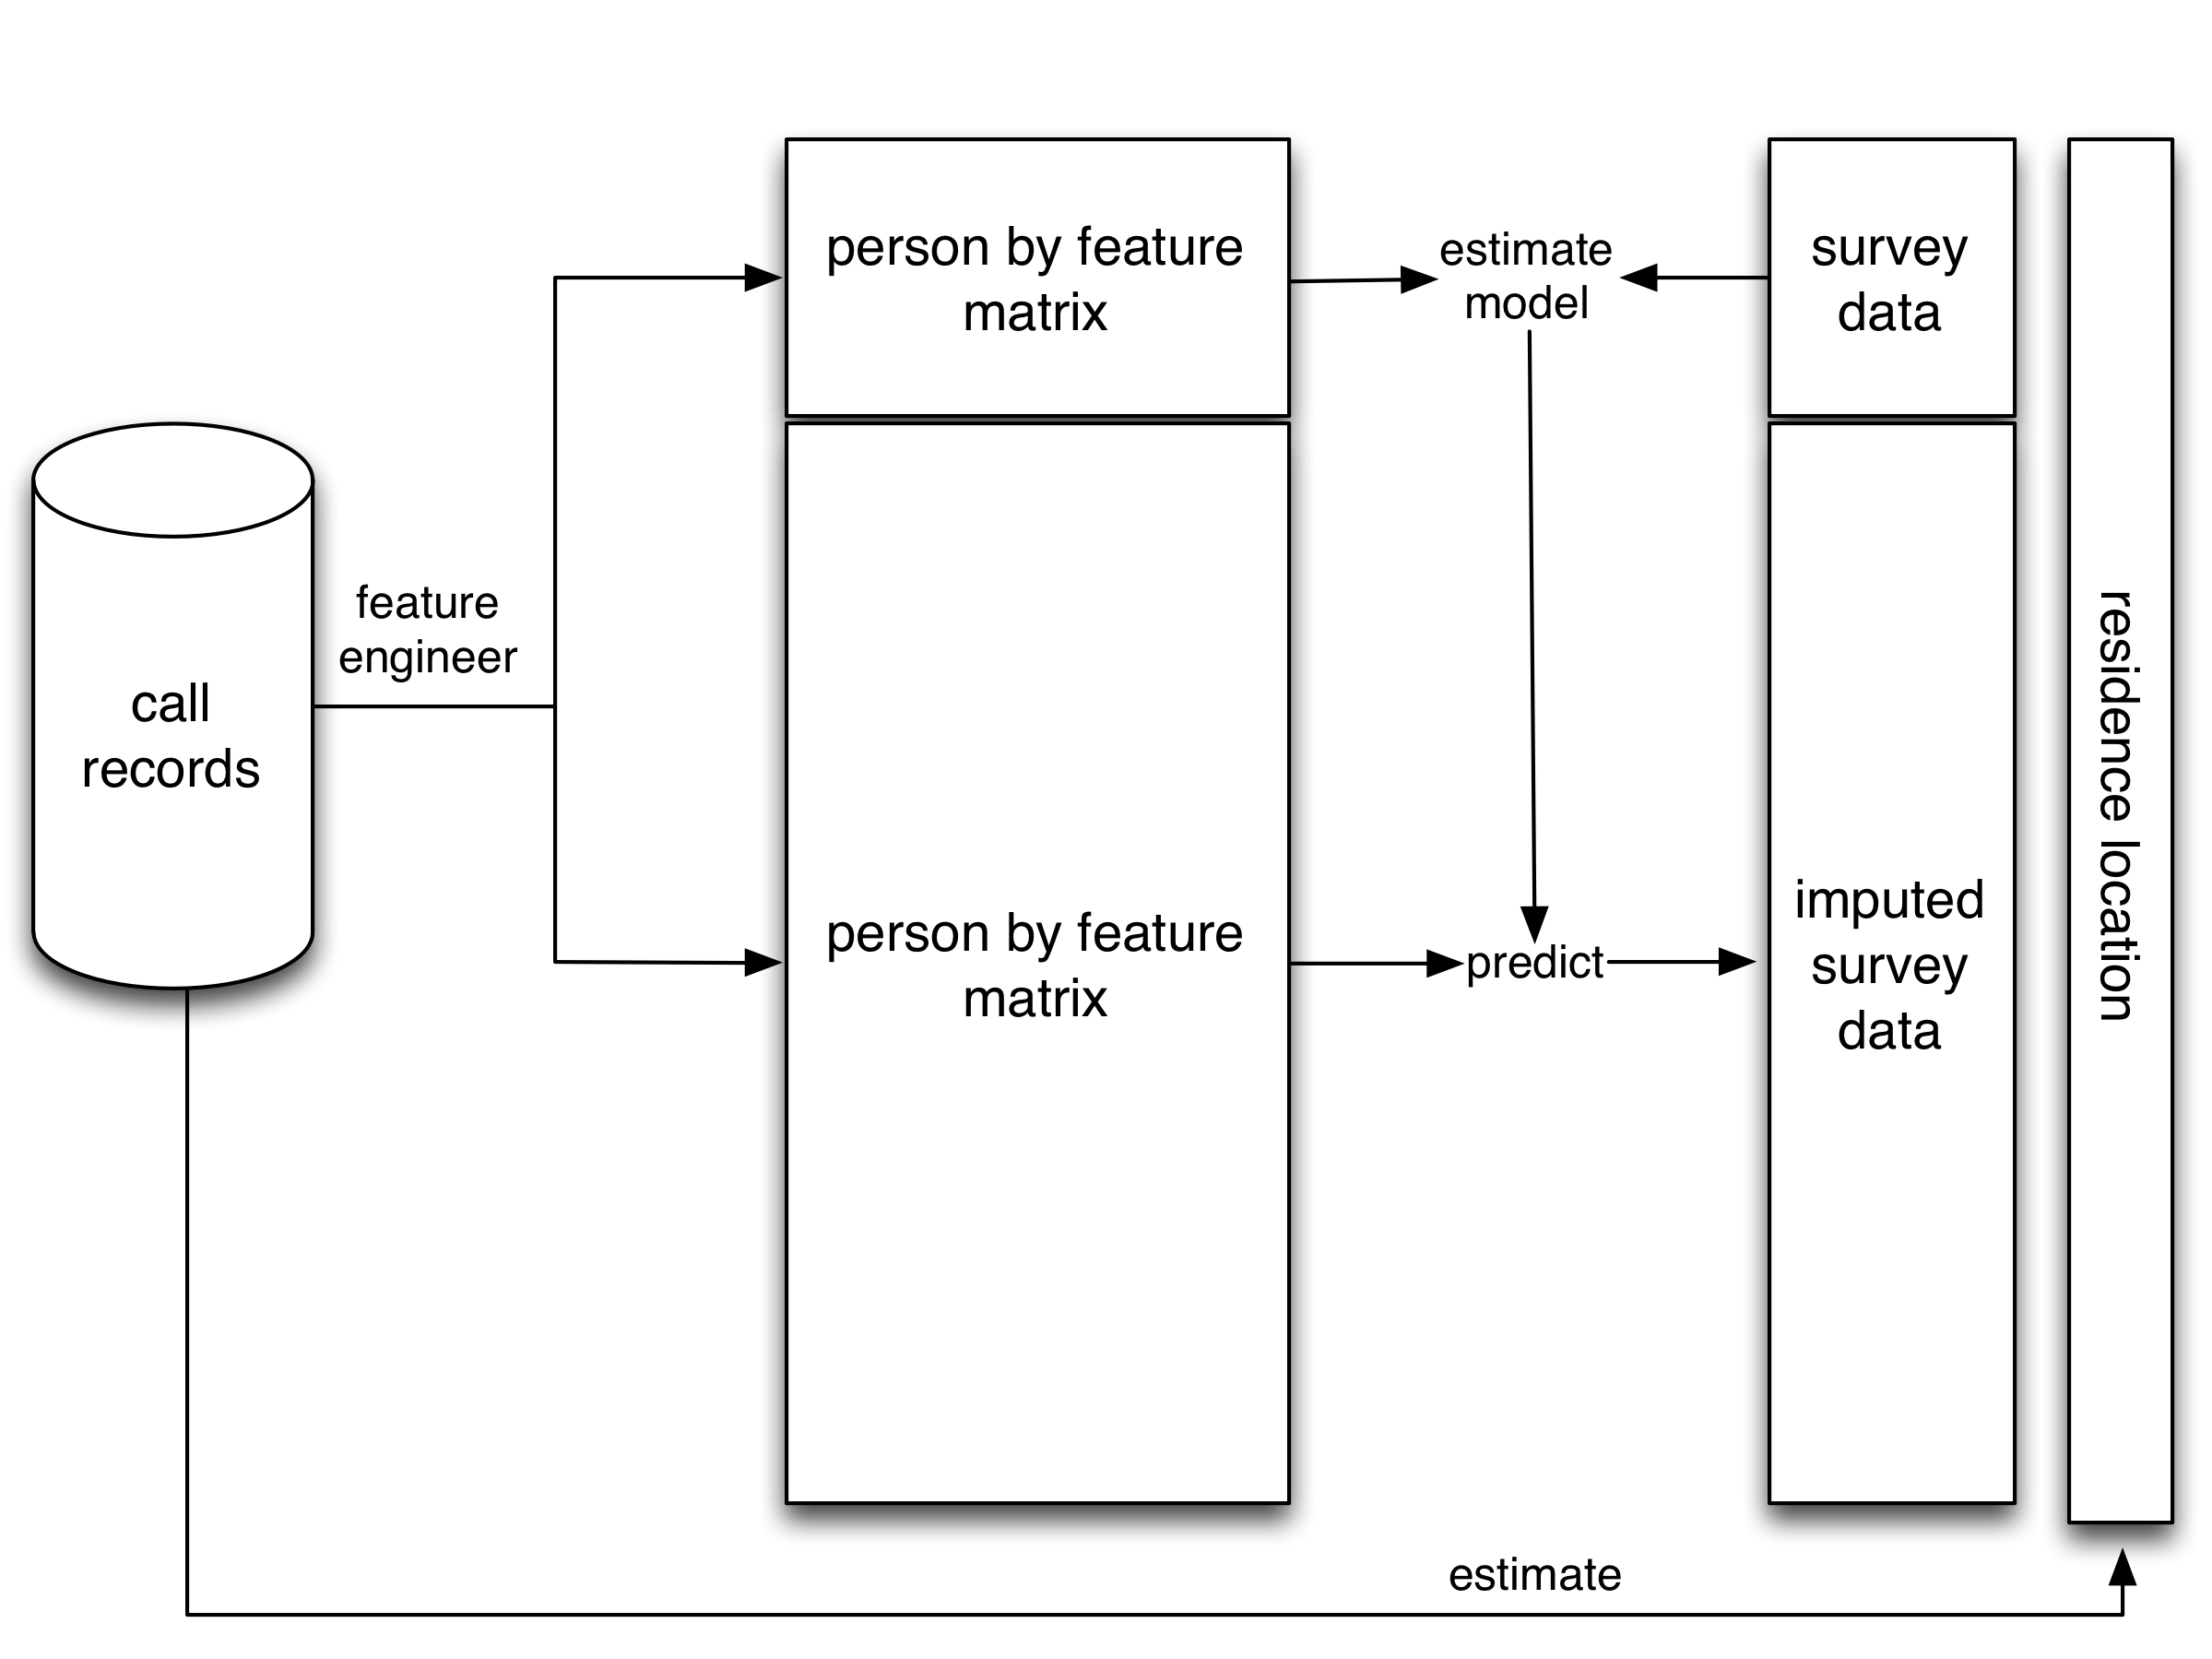
\includegraphics[width=0.7\textwidth]{figures/blumenstock_predicting_2015_schematic_6}
\end{center}
\vfill
See Chapter 3 of Salganik (2018)
\end{frame}
%%%%%%%%%%%%%%%%%%%%%%%%%%%
\begin{frame}

\begin{center}
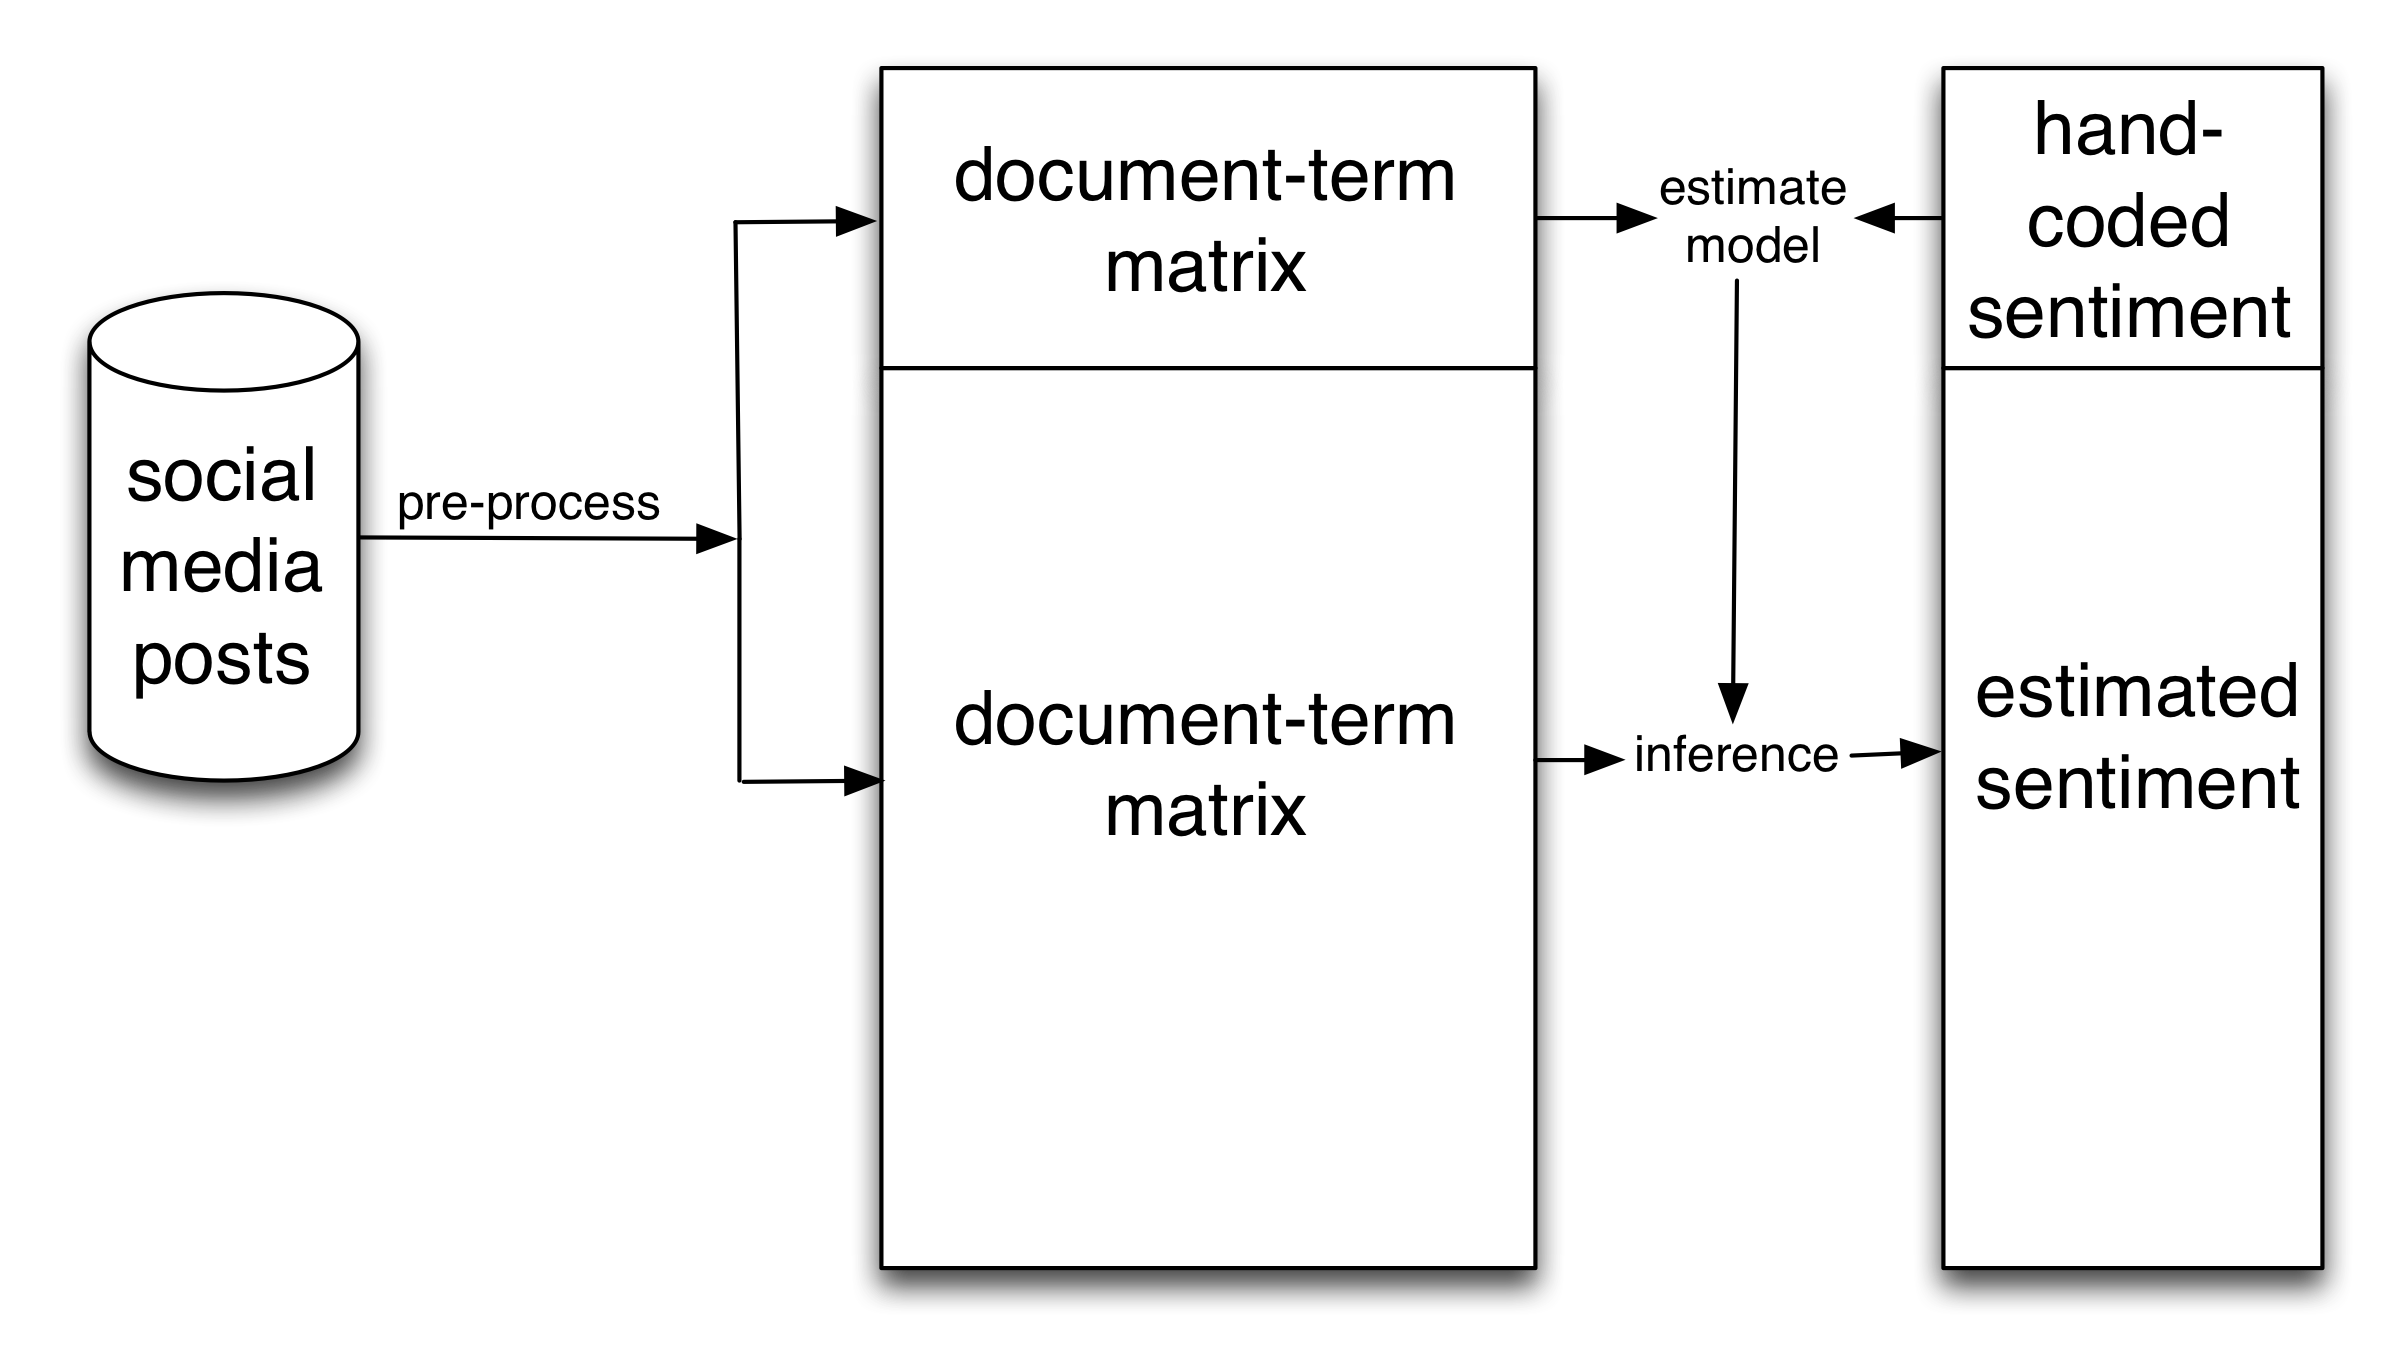
\includegraphics[width=0.9\textwidth]{figures/king_how_2013_schematic}
\end{center}
\vfill
See Chapter 2 of Salganik (2018)
\end{frame}
%%%%%%%%%%%%%%%%%%%%%%%%%%%
\begin{frame}

\begin{center}
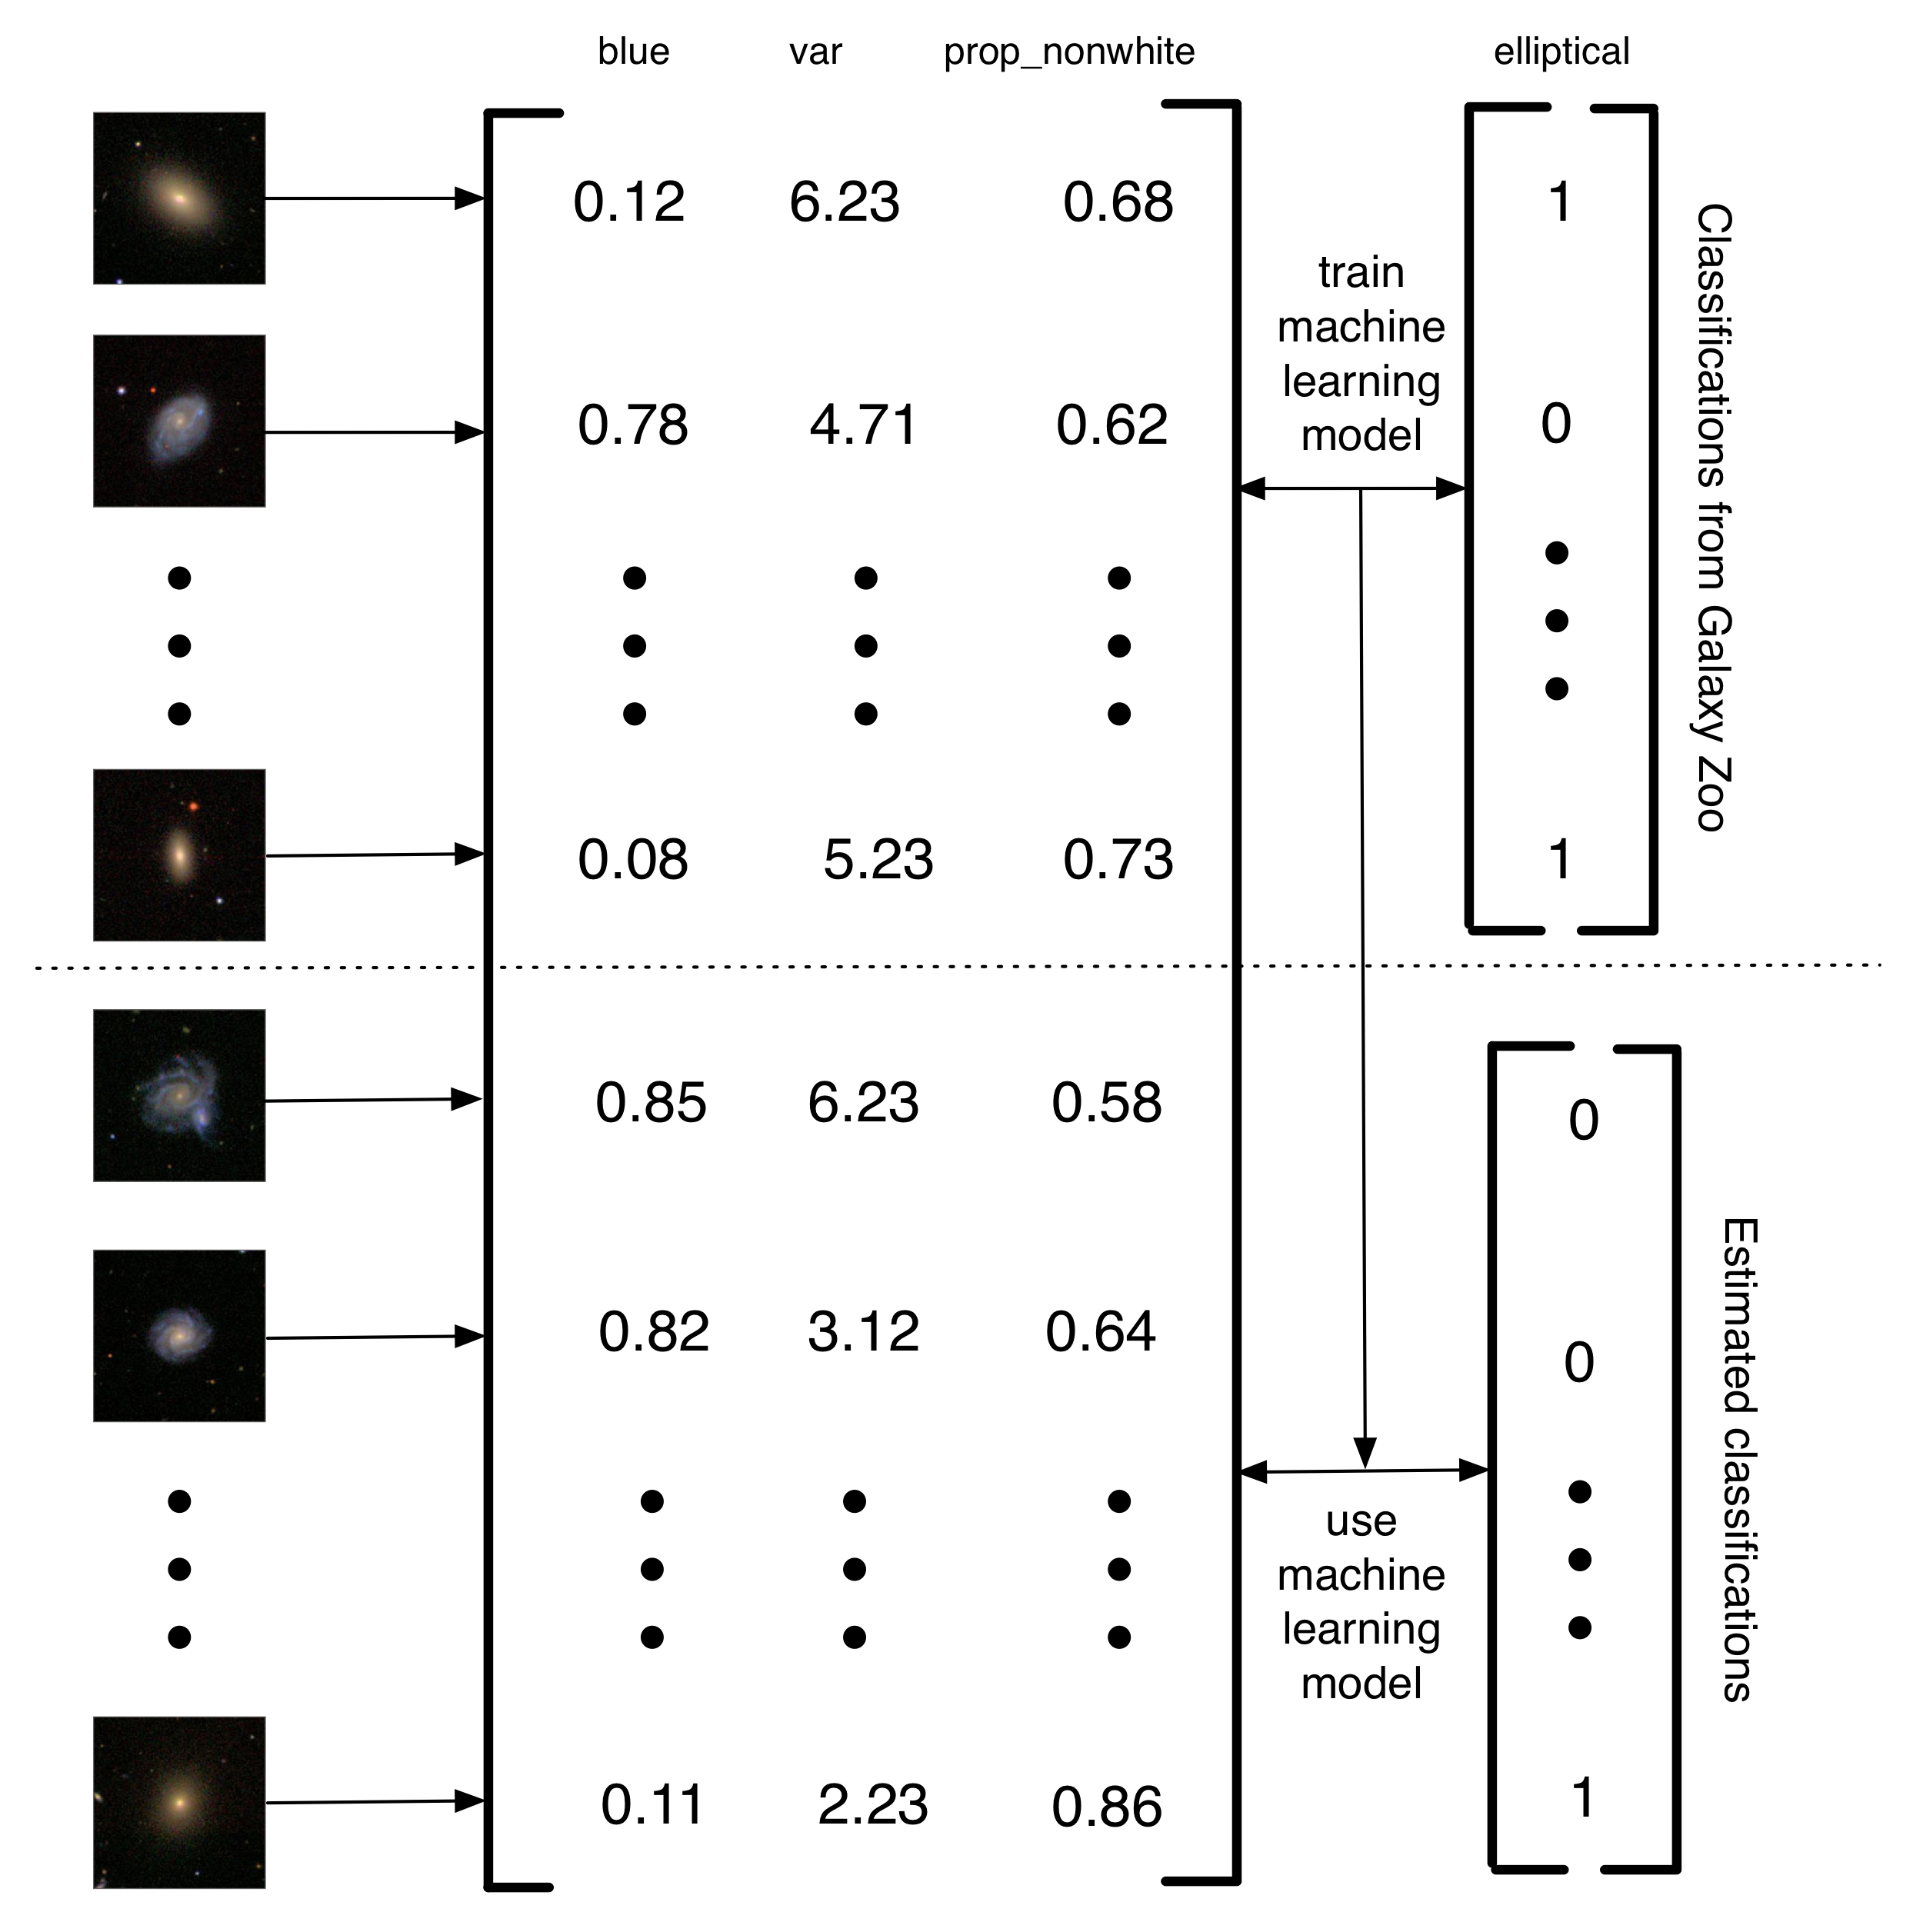
\includegraphics[height=0.9\textheight]{figures/gz_banerji_schematic}
\end{center}
\vfill
See Chapter 5 of Salganik (2018)
\end{frame}
%%%%%%%%%%%%%%%%%%%%%%%%%%%
\begin{frame}

Supervised learning:\\
Lots of input-output pairs; goal is to develop a function that will predict the output from the input

\end{frame}
%%%%%%%%%%%%%%%%%%%%%%%%
\begin{frame}

\Large{
\begin{center}
What if rather than engineering the features you could ``learn'' them automatically?
\end{center}
}
\end{frame}
%%%%%%%%%%%%%%%%%%%%%%%%
\begin{frame}

\begin{center}
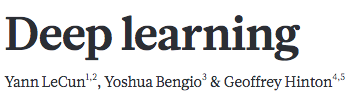
\includegraphics[width=0.8\textwidth]{figures/lecunn_deep_2015}
\end{center}
\vfill
\url{http://dx.doi.org/10.1038/nature14539}

\end{frame}
%%%%%%%%%%%%%%%%%%%%%%%%%%%
\begin{frame}

\begin{center}
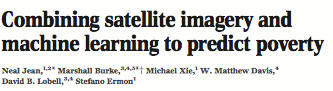
\includegraphics[width=0.6\textwidth]{figures/jean_combining_2016_title}
\end{center}

\pause

\begin{center}
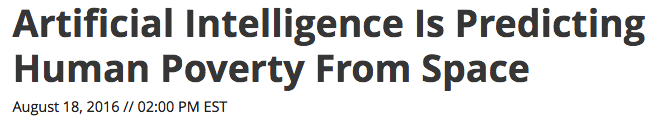
\includegraphics[width=0.6\textwidth]{figures/vice_headline.png}
\end{center}

\vfill
\url{http://dx.doi.org/10.1126/science.aaf7894}\\
\url{https://motherboard.vice.com/en_us/article/artificial-intelligence-is-predicting-human-poverty-from-space}

\end{frame}
%%%%%%%%%%%%%%%%%%%%%%%%%%%
\begin{frame}

Live demo:
\url{https://www.google.com/maps/place/Kigali,+Rwanda/@-1.9546259,30.0345059,26517m/data=!3m2!1e3!4b1!4m5!3m4!1s0x19dca4258ed8e797:0xf32b36a5411d0bc8!8m2!3d-1.9705786!4d30.1044288}

\end{frame}
%%%%%%%%%%%%%%%%%%%%%%%%%%%
\begin{frame}

But, most people had been using night lights
\begin{center}
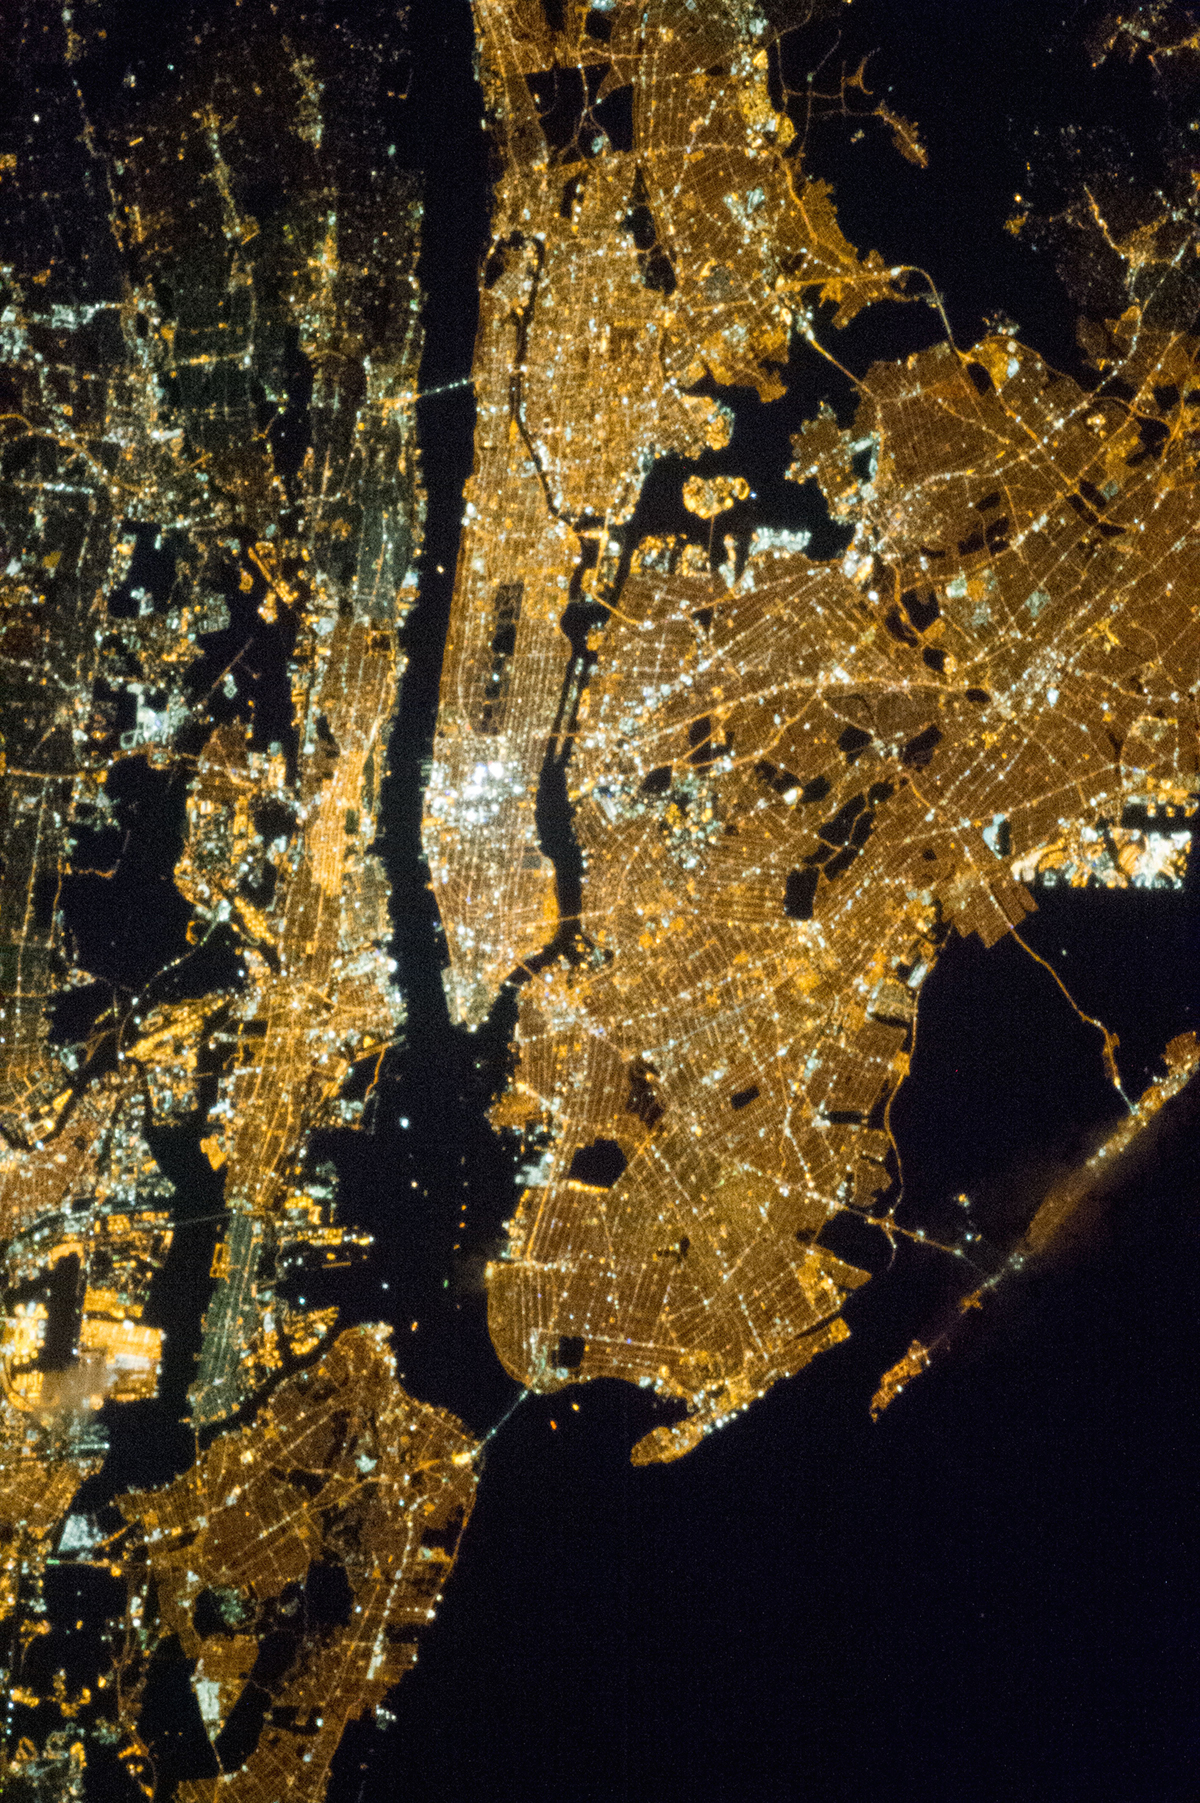
\includegraphics[height=0.7\textheight]{figures/nyc_night}
\end{center}

\vfill
\url{https://www.nasa.gov/multimedia/imagegallery/image_feature_2480.html}
\end{frame}
%%%%%%%%%%%%%%%%%%%%%%%%%%%
\begin{frame}

Prior research:\\
Nightlights + survey data to estimate wealth in places without surveys

\end{frame}
%%%%%%%%%%%%%%%%%%%%%%%%%%%
\begin{frame}

Jean et al. (2016):\\
Day pictures + Nightlights + survey data to estimate wealth in places without surveys

\end{frame}
%%%%%%%%%%%%%%%%%%%%%%%%%%%
\begin{frame}

\begin{center}
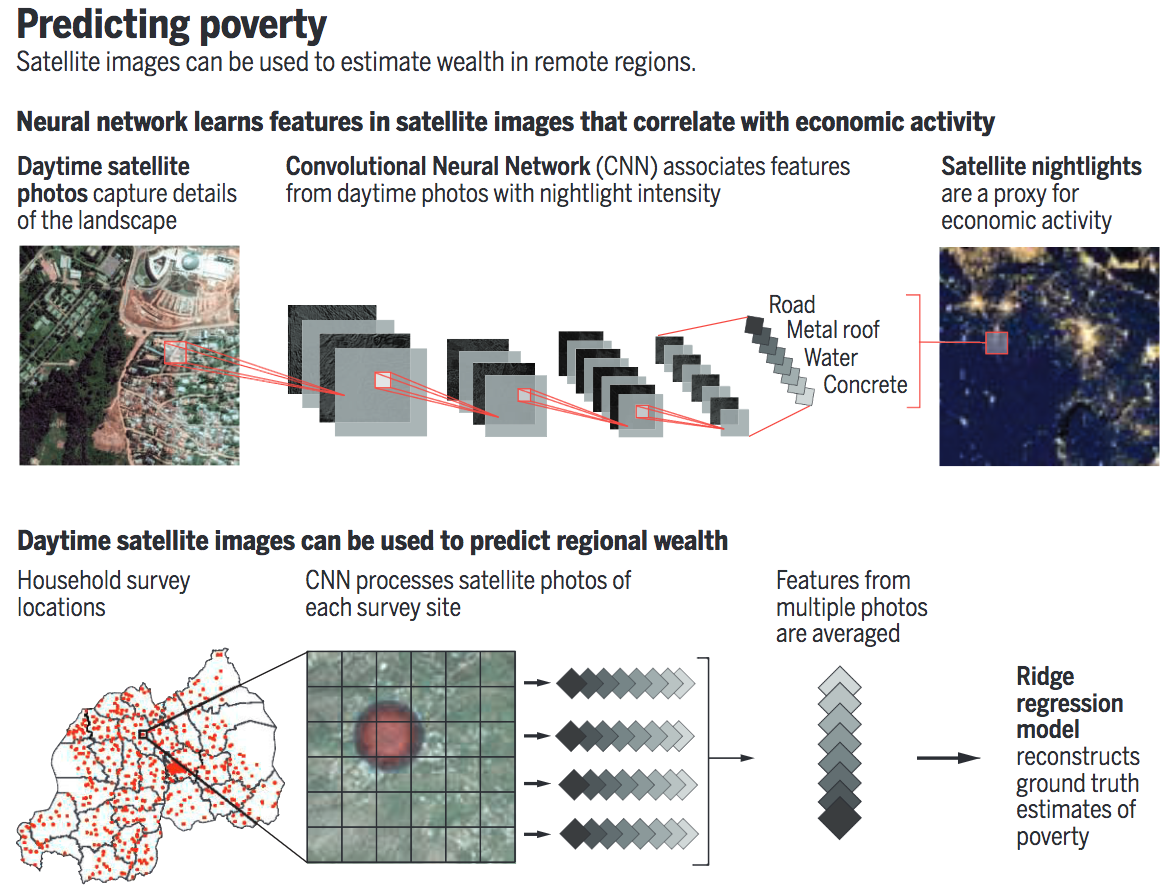
\includegraphics[width=0.4\textwidth]{figures/blumenstock_fighting_2016_fig}
\end{center}

\begin{itemize}
\item Start with CNN pretrained on ImageNet (e.g. hampsters and weasels)
\pause
\item Train CNN to predict nightlights from day pictures (lots of training data)
\end{itemize}

\end{frame}
%%%%%%%%%%%%%%%%%%%%%%%%%%%
\begin{frame}

\begin{center}
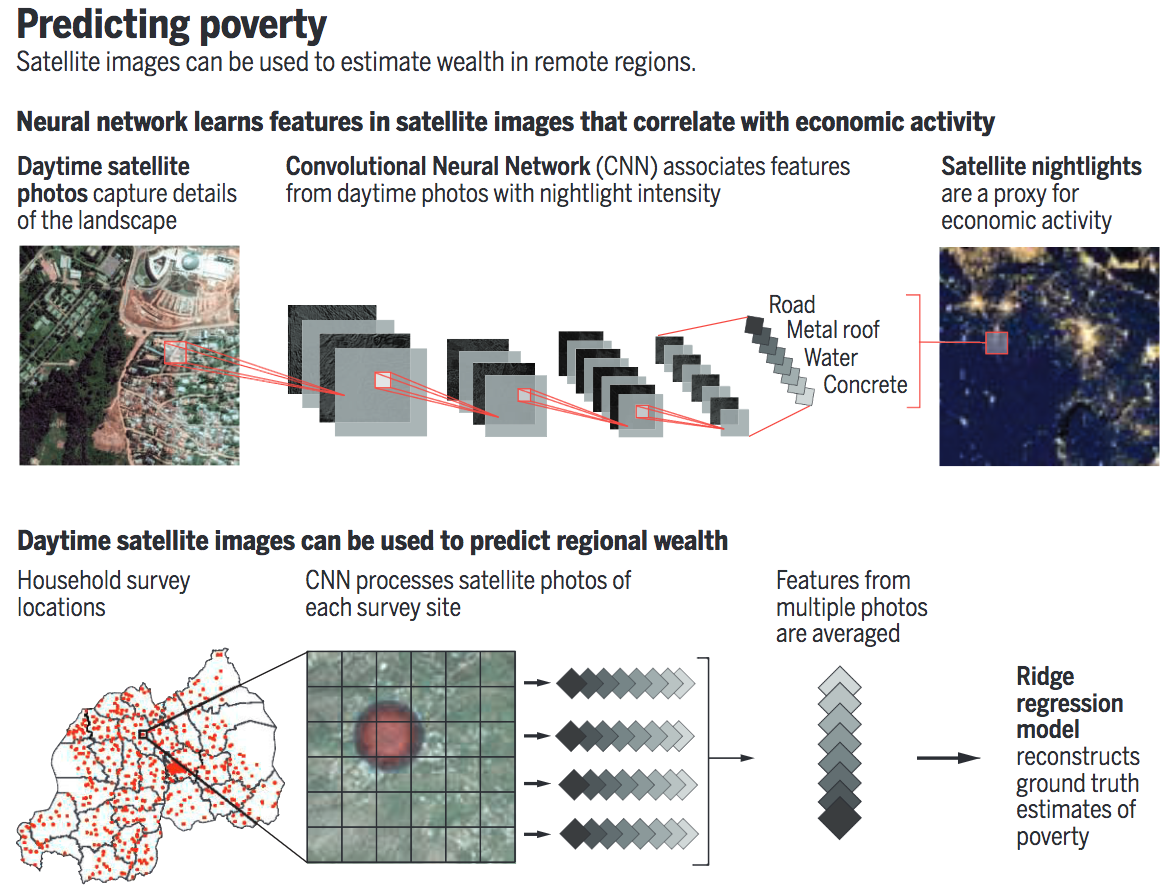
\includegraphics[width=0.4\textwidth]{figures/blumenstock_fighting_2016_fig}
\end{center}

\begin{itemize}
\item Start with CNN pretrained on ImageNet (e.g. hampsters and weasels)
\item Train CNN to predict nightlights from day pictures (lots of training data)
\item Take features from CNN and train ridge regression to predict cluster mean survey response
\end{itemize}

\vfill

\url{http://dx.doi.org/10.1126/science.aah5217}
\end{frame}
%%%%%%%%%%%%%%%%%%%%%%%%%%%
\begin{frame}

\begin{center}
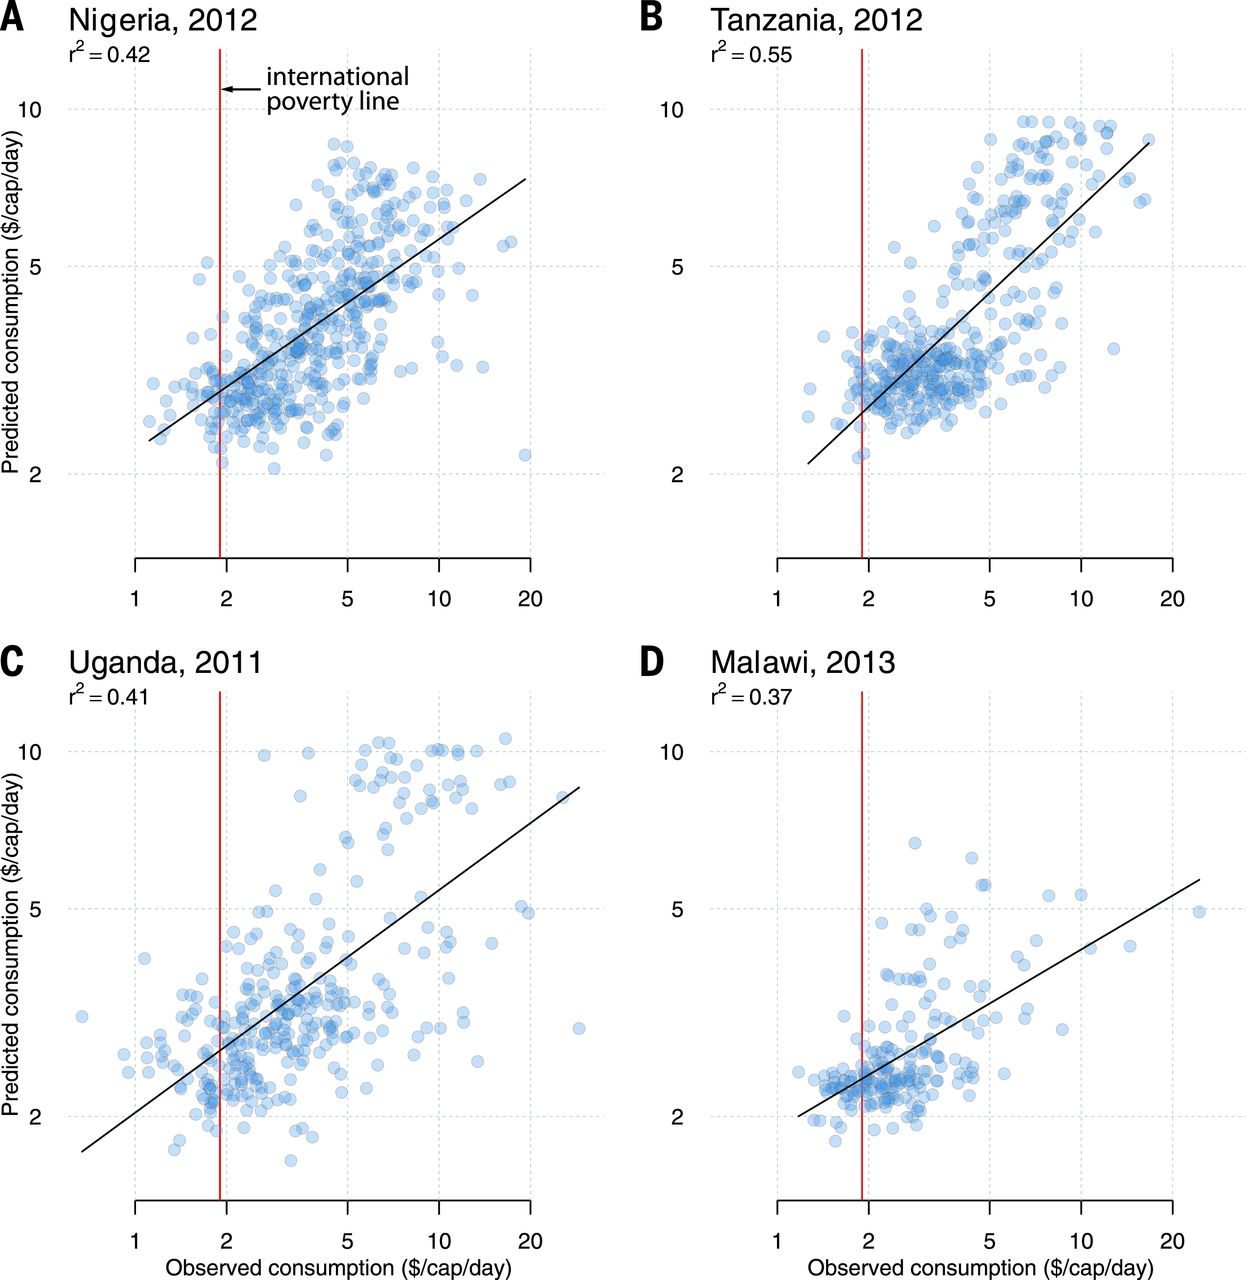
\includegraphics[width=0.5\textwidth]{figures/jean_combining_2016_fig3}
\end{center}

\end{frame}
%%%%%%%%%%%%%%%%%%%%%%%%%%%
\begin{frame}

\begin{center}
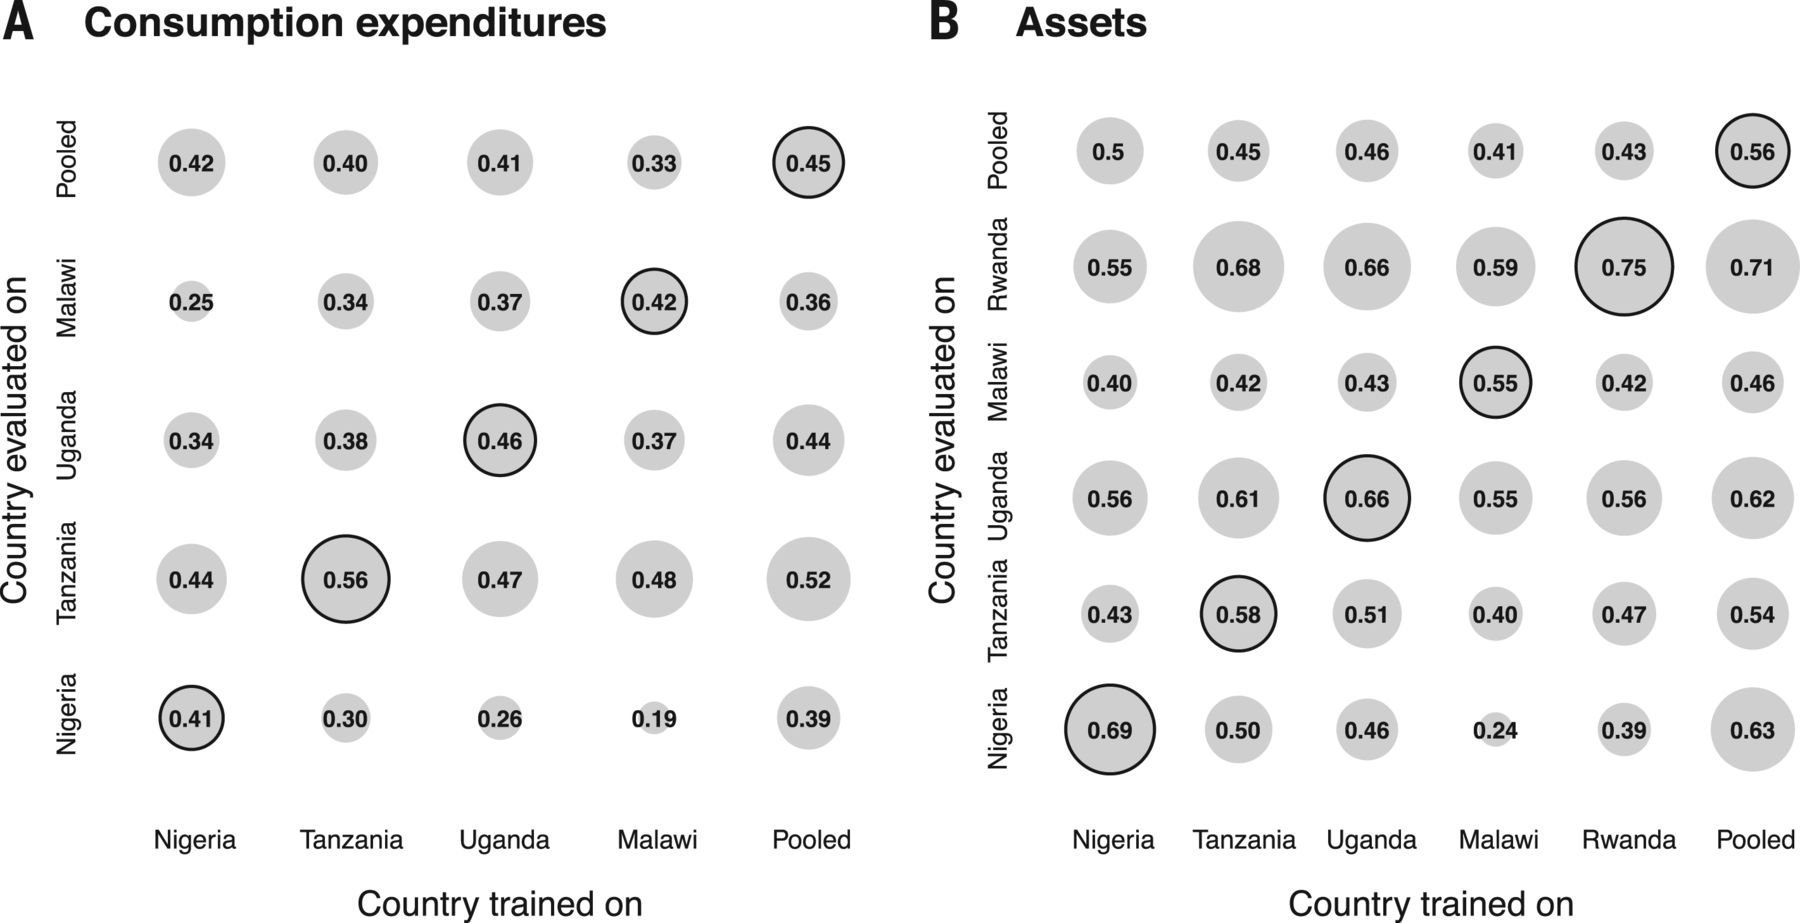
\includegraphics[width=0.9\textwidth]{figures/jean_combining_2016_fig5}
\end{center}

\end{frame}
%%%%%%%%%%%%%%%%%%%%%%%%%%%
\begin{frame}

\begin{center}
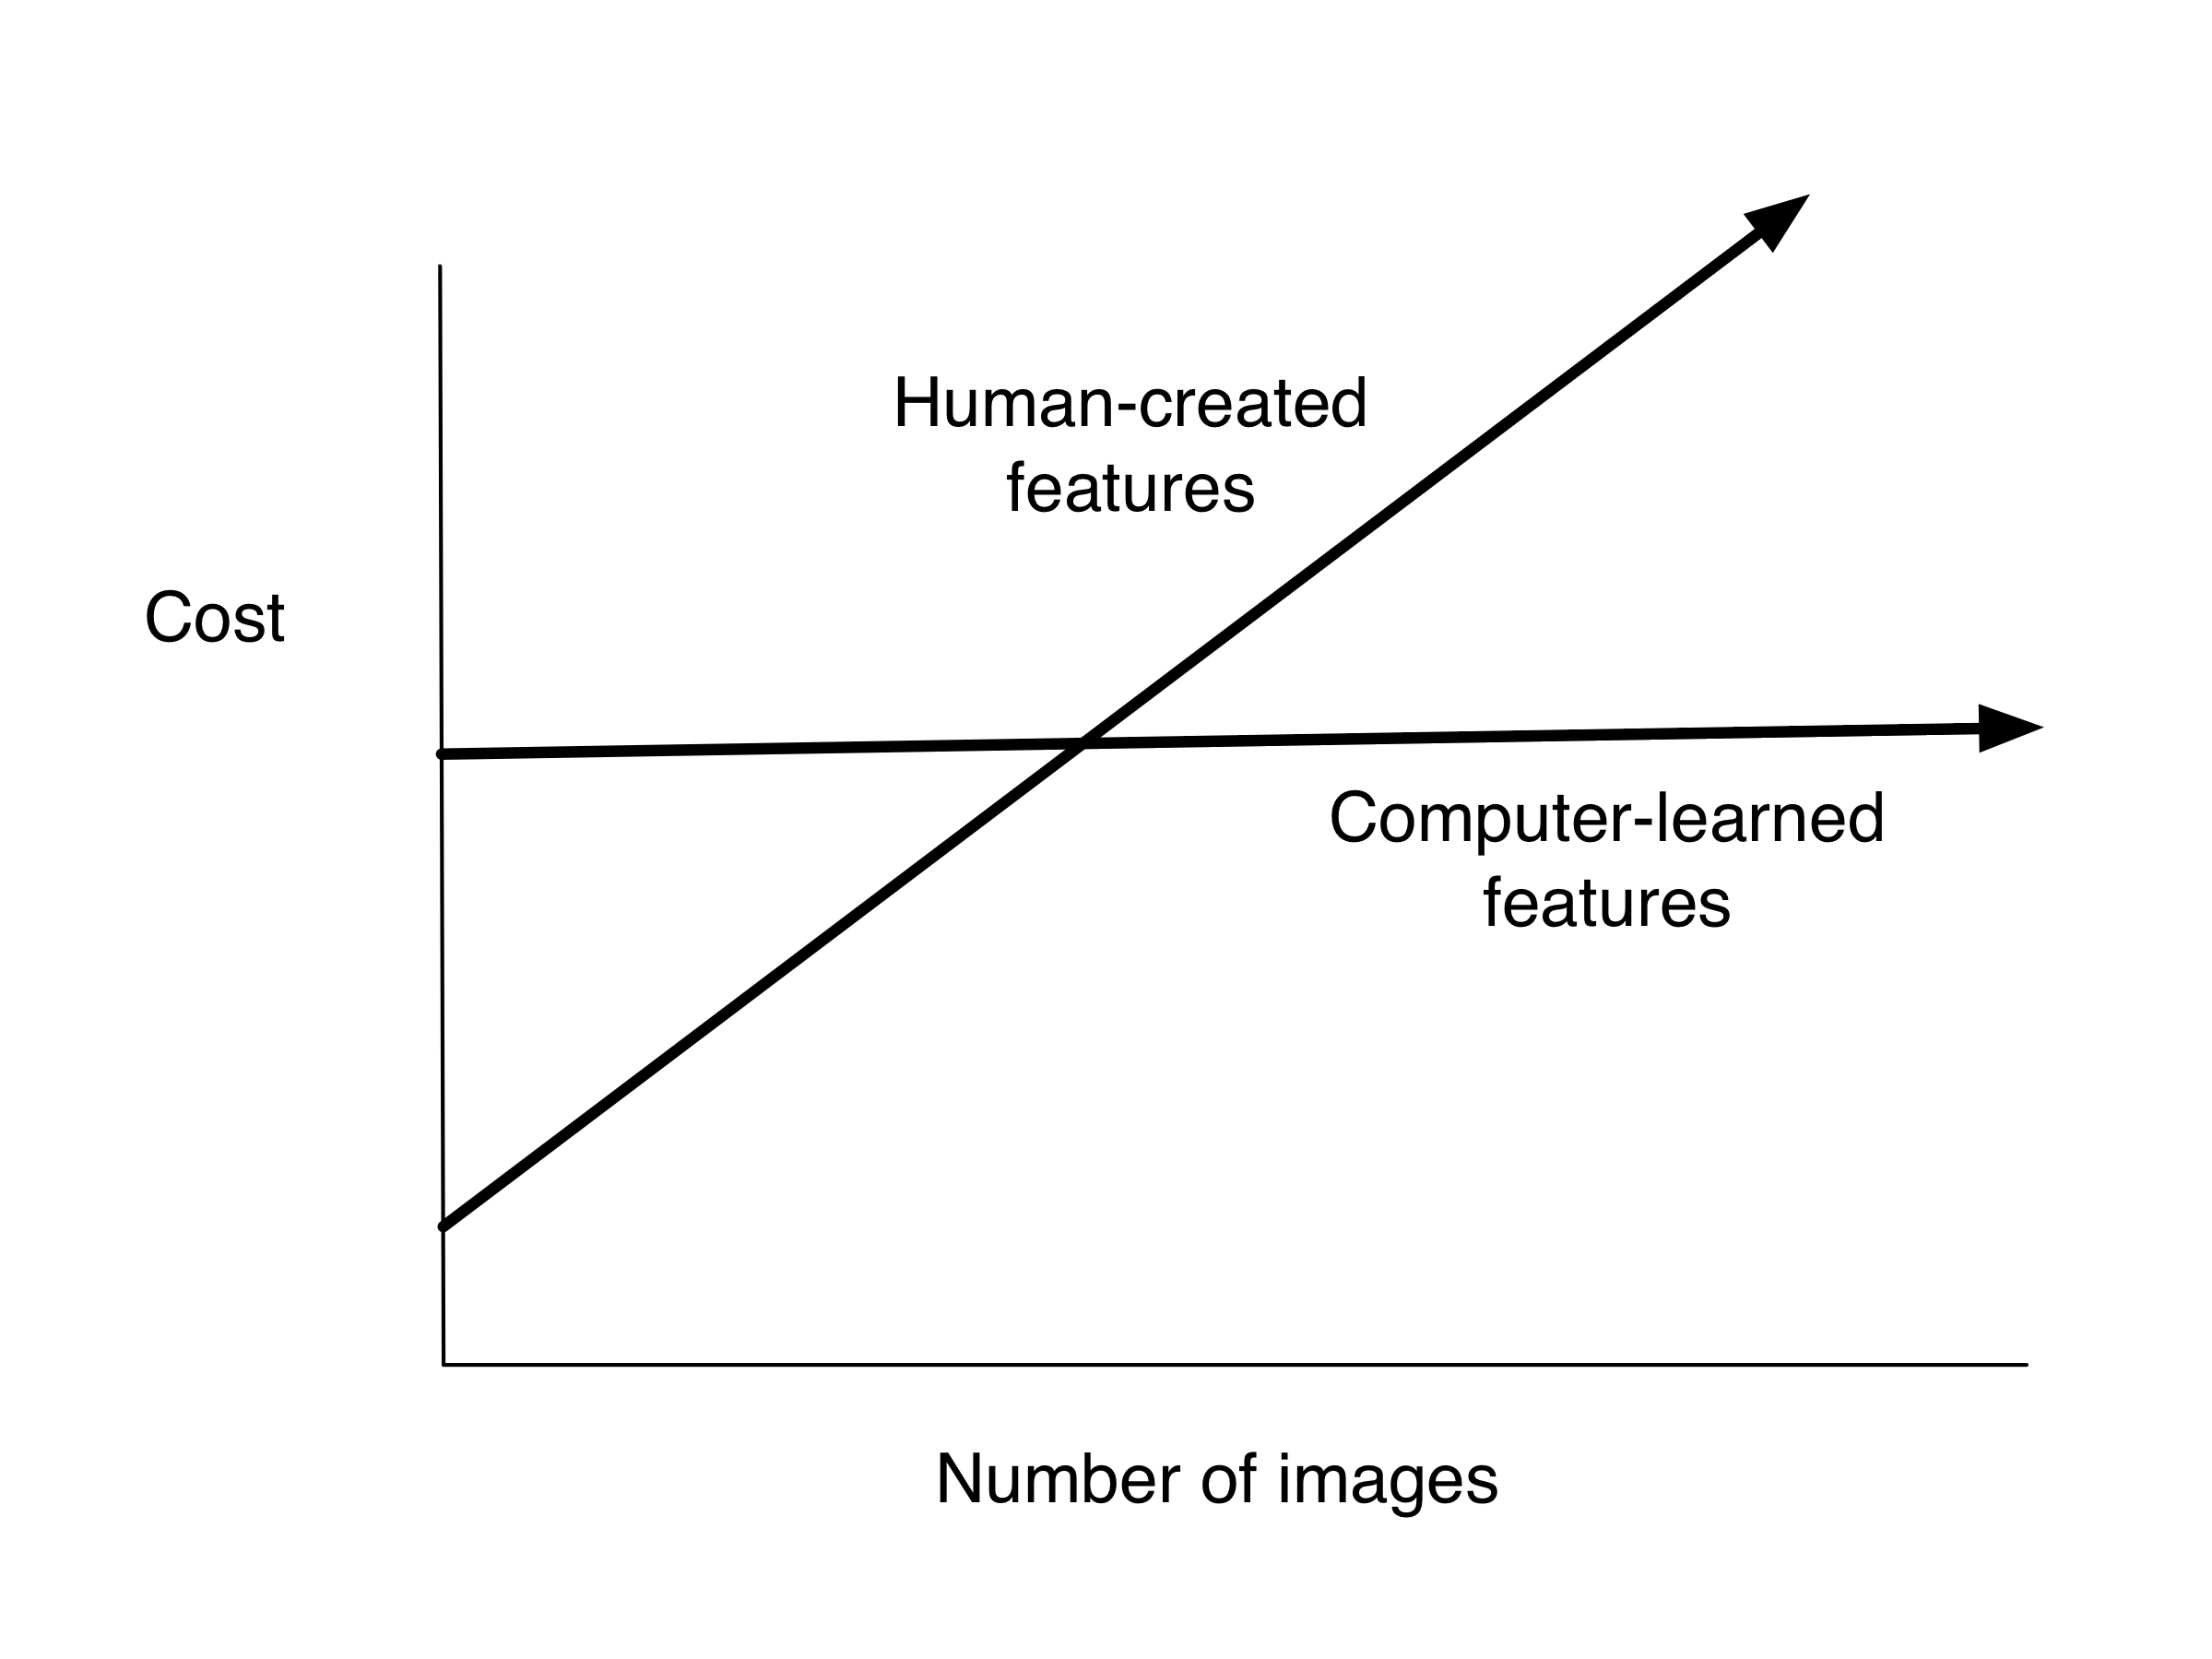
\includegraphics[width=0.7\textwidth]{figures/zero_variable_cost_features}
\end{center}

\end{frame}
%%%%%%%%%%%%%%%%%%%%%%%%%%%
\begin{frame}

\begin{center}
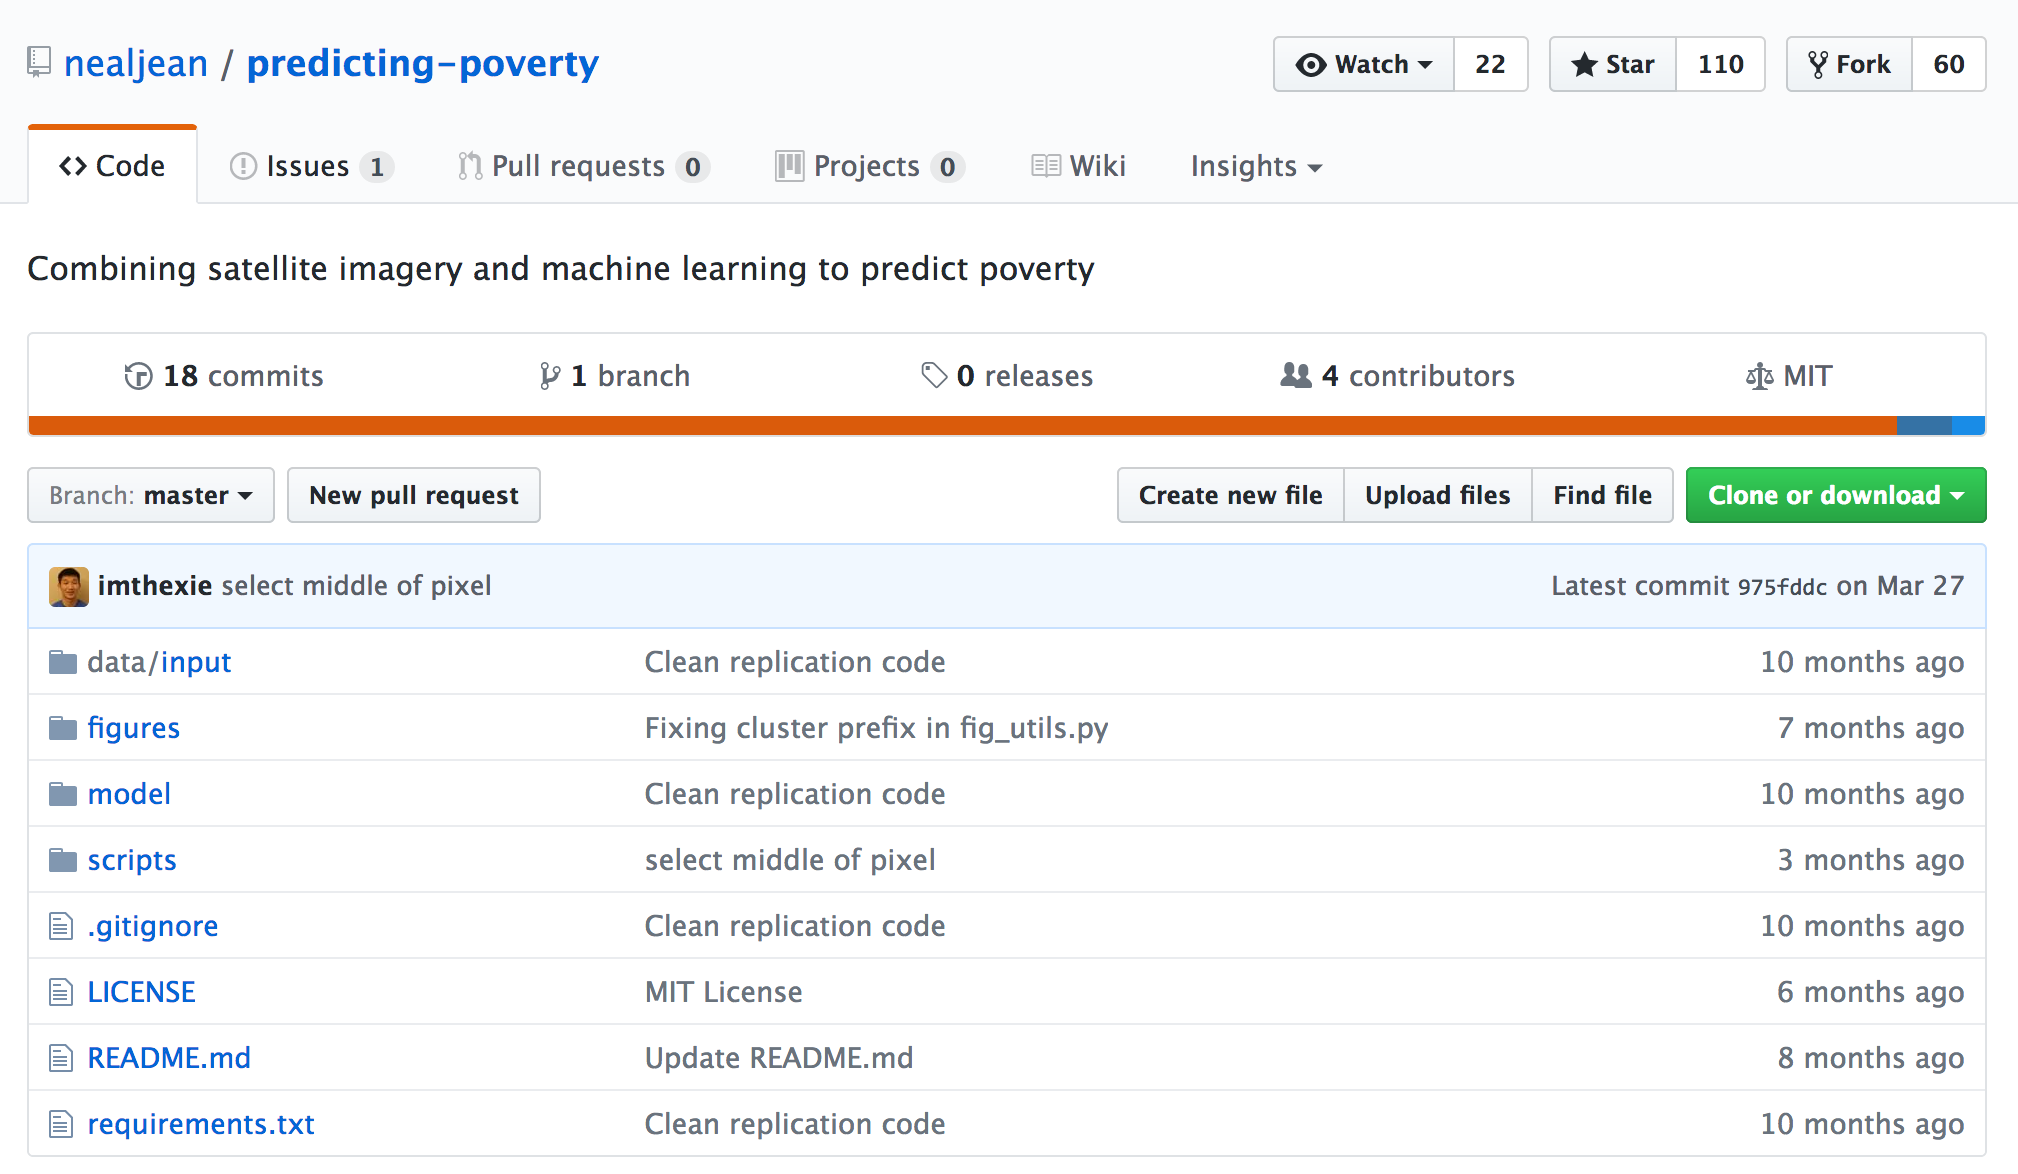
\includegraphics[width=0.7\textwidth]{figures/jean_predicting_github}
\end{center}

\vfill
\url{https://github.com/nealjean/predicting-poverty}

\end{frame}
%%%%%%%%%%%%%%%%%%%%%%%%%%%
\begin{frame}

Wrap-up:
\begin{itemize}
\item Surveys and big data are compliments not substitutes
\pause
\item Sometime we do ``enriched asking'' and sometimes ``amplified asking'' (role of big data source is different in both cases)
\pause
\item Learn more: see ``what to read next'' in Ch 3 of Bit by Bit.
\end{itemize}

\end{frame}
%%%%%%%%%%%%%%%%%%%%%%%%%%%

\end{document}
